Erinnern wir uns an \autoref{eq:multi_grav} aus der \nameref{ch:einl}, in welcher die gravitationelle Wechselwirkung zwischenzwei Körpern $x$ und $y$ beschrieben wurde. 
Die Struktur dieser Formel erinnert stark an Matrizen. 
Ein Ansatz, um große vollbesetzte Matrizen speicherplatzsparend aufzustellen und Berechnungen zeiteffektiv durchzuführen, besteht darin, sie als hierarchische Matrizen darzustellen.
Im Folgenden sollen daher die Grundlagen für allgemeine $\mathcal{H}$- und \hquad eingeführt werden. Für ausführlichere Arbeiten zu dem Thema der hierarchischen Matrizen verweise 
ich auf \citet{h2diss} und \citet{hackbusch1999sparse}.

\TODO{Quellenangaben einfügen: vgl. Nicht lokale Operationen}

Erarbeitet wurde das Konzept der hierarchischen Matrizen unter anderem zur effektiven Lösung Fredholmscher Integralgleichungen:
\begin{equation*}
  u\left(x\right) = \int_{\Omega} u\left(x\right) g\left(x, y\right) \forall x \in \Omega .
\end{equation*}
Dabei ist $\Omega \subseteq \R^d$ und $g \colon \R^d \times \R^d \to \R$ eine sogenannte \textit{Kernfunktion}.
Diskretisiert man diese Gleichung mit dem Galerkinverfahren unter Verwendung einer Finite-Elemente-Basis $\left(\phi_i\right)_{i \in I}$ erhält man die zugehörige Matrix
\begin{equation*}
  G_{ij} = \int_{\Omega} \int_{\Omega} \phi_i\left(x\right) g\left(x,y\right) \phi_j\left(y\right) \ dy \ dx ,\quad \forall i, j \in I.
\end{equation*} 
Um die Integration über $\Omega \times \Omega$ aufspalten zu können, ist es notwendig, dass die Variablen in der Kernfunktion getrennt werden können.
Die Kernfunktion $g$ muss also in der Form
\begin{equation*}
  g\left(x,y\right) = \sum_{\nu \in \haken{k}} a_{\nu}\left(x\right) b_{\nu}\left(y\right)
\end{equation*}
mit $k \in \N$, $a_{\nu}, b_{\nu} \colon \R^d \to \R$ vorliegt. Eine Kernfunktion dieser Form heißt \textit{entartete Kernfunktion} von Rang k.
Allgemein nennen wir eine Funktion $g$ eine Kernfunktion einer Matrix $G$, falls die Funktion $g$ die Matrix $G$ erzeugt, also gerade $G_{\mu\nu} = g{\mu, \nu}$ gilt.
Nicht jede Kernfunktion ist entartet, es lassen sich aber oft entartete Kernfunktionen konstruieren, die die Funktion approximieren. Möglichkeiten sind beispielsweise
Approximationen durch Taylor-Entwicklung oder Interpolation. \citep{h2diss}

Seien $X, Y$ Mengen und $G \in \R^{X \times Y}$ eine Matrix mit Kernfunkion $g \colon X \times Y \to \R$. Ist $g$ entartet, so gilt also für $x \in X$ und $y \in Y$ 
gerade $G_{xy} = g\left(x, y\right) = \sum_{\nu \in \haken{k}} a_{\nu}\left(x\right) b_{\nu}\left(y\right)$. Die Summe in dieser Gleichung können wir auch durch Multiplikation zweier Matrizen $A \in \R^{X \times k}$ und 
$\trans{B} \in \R^{Y \times k}$ mit $A_{x\nu} = a_{\nu}\left(x\right)$, $B_{y\nu} = b_{\nu}\left(y\right)$ ausdrücken. Analog dazu, die Kernfunktion als entartete Kernfunktion darzustellen, ist also die Darstellung der Matrix
$G$ durch Matrizen $A$ und $B$ durch $G = A\trans{B}$.
    
    \subsubsection{Approximation}
    \label{sec:approx}
      Im Folgenden möchte ich eine beispielhafte Approximation einer nicht-entarteten Kernfunktion durch Interpolation vorstellen, um so eine entartete Kernfunktion zu erhalten.
      Der Aufbau folgt weitestgehend dem von \citet{nichtlokop}. Für eine Approximation einer nicht-entarten Kernfunktion durch Taylor-Entwicklung verweise ich auf \citet{h2diss}. 
      
      Sei $g \colon \Omega \times \Omega \to \R$ eine nicht-entartete Kernfunktion. Für eine Interpolationsordnung $k$ und ein Teilgebiet $\sigma \subset \Omega$ wählen wir Interpolationspunkte 
      $\xi_\inds{1}, \dots , \xi_\inds{k}$. Nun suchen wir eine Approximation von $\left. g\right|_{\Omega \times \sigma}$ der Form
      \begin{equation}
      \label{eq:gsigma}
	g_\sigma\left(x, y\right) = \sum_{\nu \in \haken{k}} g\left(x, \xi_\inds{\nu}\right) \lag_\inds{\nu}\left(y\right),
      \end{equation}
      in der $x$ und $y$ getrennt sind. Somit hätten wir bereits eine entartete Kernfunktion. In eben dieser Form werden Lagrange-Interpolaten in Stützstellen 
      $\xi_\inds{\nu}$ mit Lagrange-Basisfunktionen $\lag_\inds{\nu}$ dargestellt. 
      
    \subsubsection{Lagrange-Interpolation im mehrdimensionalen Raum}
      Bevor wir die Funktion $g$ wie in \autoref{eq:gsigma} approximieren können, müssen wir die Lagrange-Basisfunktionen auf mehrdimensionalen Gebieten konstruieren und einige 
      Eigenschaften sicherstellen. 
      Zunächst definieren wir dazu die Lagrange-Basispolynome auf dem Referenzintervall $[-1,1]$. Für $k \in \N$, $\nu \in \nullhaken{k}$ und paarweise verschiedene Stützstellen
      $\xi_0, \dots , \xi_k \in [-1,1]$ ist durch
      \begin{equation*}
	\lag_\nu\left(x\right) := \prod_{\substack{\mu \in \nullhaken{k} \\ \mu \neq \nu}} \frac{x - \xi_\mu}{\xi_\nu - \xi_\mu} \ \ \ \ \ \ \ \ \ \ \ \  \text{für alle } x \in [-1,1]
      \end{equation*}
      das $\nu$-te Lagrange-Polynom gegeben.
      Eine Eigenschaft der Lagrange-Polynome, die wir später noch benötigen, ist:
      \begin{equation}
	\lag_\nu\left(\xi_\mu\right) = \delta_{\nu\mu} =
	\begin{cases}
	  1 & \text{falls } \nu = \mu,\\
	  0 & \text{sonst.}
	\end{cases}
	\label{eq:lag_delta}
      \end{equation}
      
      Wir können durch
      \begin{equation*}
	\mathfrak{I} \colon C[-1,1] \to \Pi_k, \ \ \ \ \ \ \ \ \ \ \ \ f \mapsto \sum_{\nu \in \nullhaken{k}} f\left(\xi_\nu\right) \lag_\nu
      \end{equation*}
      einen Lagrange-Interpolationsoperator definieren, der auf $[-1,1]$ stetige Funktionen auf Polynome aus $\Pi_k$ abbildet, also auf Polynome von höchstens Grad $k$.
      
      Um diesen Operator auf Funktionen auf beliebigen Intervallen $[a,b]$ mit $a < b$ zu übertragen, definieren wir eine Transformation
      \begin{equation*}
	\Phi_{[a,b]} \colon [-1,1] \to [a,b] \ \ \ \ \ \ \ \ \ \ \ \  x \mapsto \frac{b + a}{2} + \frac{b - a}{2} x,
      \end{equation*}
      die für alle $x \in [-1,1]$ die Eigenschaften
      \begin{equation*}
	\Phi_{[a,b]}\left(-1\right) = a , \ \ \ \ \Phi_{[a,b]}\left(1\right) = b , \ \ \ \ \Phi'_{[a,b]}\left(x\right) = \frac{b - a}{2} > 0
      \end{equation*}
      hat, also affin und bijektiv ist. Für $f \in C[a,b]$ gilt also $\tilde f := f \after \Phi_{[a,b]} \in C[-1,1]$, sodass wir den auf $[-1,1]$ definierten Interpolationsoperator $\mathfrak{I}$
      auf $\tilde f$ anwenden können. Wir können also einen Interpolationsoperator auf dem Intervall $[a,b]$ durch
      \begin{equation*}
	\mathfrak{I}_{[a,b]} \colon C[a,b] \to \Pi_k, \ \ \ \ \ \ \ \ \ \ \ \ f \mapsto \mathfrak{I}[f \after \Phi_{[a,b]}] \after \Phi_{[a,b]}^{-1}
      \end{equation*}
      definieren, was, die Definition von $\mathfrak{I}$ eingesetzt, die Darstellung
      \begin{equation*}
	\mathfrak{I}_{[a,b]}[f] = \sum_{\nu \in \nullhaken{k}} f \after \Phi_{[a,b]}\left(\xi_\nu\right) \lag_\nu \after \Phi_{[a,b]}^{-1} = 
				 \sum_{\nu \in \nullhaken{k}} f \left( \Phi_{[a,b]}\left(\xi_\nu\right)\right)     \lag_\nu \after \Phi_{[a,b]}^{-1}
      \end{equation*}
      ergibt.
      
      Zur Vereinfachung definieren wir für $\nu \in \nullhaken{k}$ und $x \in [a,b]$
      \begin{align*}
	\xi_{[a,b],  \nu} &:= \Phi_{[a,b]}\left(\xi_\nu\right) = \frac{b + a}{2} + \frac{b - a}{2} \xi_\nu\\
	\lag_{[a,b], \nu} &:= \prod_{\substack{\mu \in \nullhaken{k} \\ \mu \neq \nu}} \frac{x - \xi_{[a,b],  \mu}}{\xi_{[a,b],  \nu} - \xi_{[a,b],  \mu}}.
      \end{align*}
      Da mit \autoref{eq:lag_delta} folgende Gleichung für alle $\nu,\mu \in \nullhaken{k}$ gilt
      \begin{align*}
	 \lag_\nu \after \Phi_{[a,b]}^{-1}\left(\xi_{[a,b],\mu}\right) &= \lag_\nu \after \Phi_{[a,b]}^{-1} \left( \Phi_{[a,b]}\left(\xi_{[a,b],\mu}\right) \right)\\
							    &= \lag_\nu \left(\xi_\mu\right) = \delta_{\nu\mu}\\
							    &= \lag_{[a,b],\nu}\left( \xi_{[a,b],\mu} \right),
      \end{align*}
      stimmen $\lag_\nu \after \Phi_{[a,b]}^{-1}$ und $\lag_{[a,b],\nu}$ in $k+1$ Punkten überein. Da beides Polynome in $\Pi_k$ sind, müssen sie identisch sein und wir erhalten die vereinfachte
      Darstellung
      \begin{equation*}
	\mathfrak{I}_{[a,b]}[f] = \sum_{\nu \in \nullhaken{k}} f\left(\xi_{[a,b],\nu}\right) \lag_{[a,b],\nu}, \ \ \ \ \ \ \ \ \ \ \ \ \text{für alle } f \in C[a,b].
      \end{equation*}
      
      
      Nun müssen wir für unser Problem noch Interpolationsoperatoren auf Gebieten im mehrdimensionalen Raum definieren. Der Einfachheit halber, und weil der später vorgestellte Algorithmus ohnehin 
      mit solchen sogenannten \wlabel{\textit{bounding boxes}}{w:bbox} arbeitet, beschränken wir uns auf achsenparallele Quader $Q = [a_1,b_1] \times \dots \times [a_d,b_d]$. Sei also eine zu interpolierende Funktion
      $f \in C\left(Q\right)$ gegeben. Für $\iota \in \haken{d}$ und $x \in Q$ gewinnen wir aus $f$ eine Funktion
      \begin{equation*}
	f_{x,\iota} \colon [a_\iota,b\iota] \to \R, \ \ \ \ \ \ \ \ \ \ \ \ y \mapsto f\left(x_1, \dots , x_{\iota-1}, y , x_{\iota+1}, \dots , x_d\right),
      \end{equation*}
      bei der alle Parameter außer dem $\iota$-ten fest sind. Auf diese Funktion auf dem Intervall $[a_\iota,b_\iota]$ können wir den Interpolationsoperator $\mathfrak{I}_{[a_\iota,b_\iota]}$ 
      anwenden und erhalten so einen Operator
      \begin{equation*}
	\mathfrak{I}_{Q,\iota} \colon C\left(Q\right) \to C\left(Q\right)
      \end{equation*}
      für den für $f \in C\left(Q\right)$ und $x \in Q$
      \begin{equation*}
	\mathfrak{I}_{Q,\iota}[f]\left(x\right) = \sum_{\nu \in \nullhaken{k}} f\left(x_1, \dots , x_{\iota-1} , \xi_{[a_\iota,b_\iota]} , x_{\iota+1}, \dots , x_d\right) \lag_{[a_\iota,b_\iota],\nu}\left(x_\iota\right)
      \end{equation*}
      gilt.
      Somit bildet $\mathfrak{I}_{Q,\iota}$ eine stetige Funktion auf eine neue stetige Funktion ab, die sich in der $\iota$-ten Komponente wie ein Polynom verhält. Durch Hintereinanderausführung
      der Operatoren für jede Dimension erhalten wir ein Polynom in jeder Komponente und mit
      \begin{equation*}
	\mathfrak{I}_Q := \mathfrak{I}_{Q,1} \after \dots \after \mathfrak{I}_{Q,d}
      \end{equation*}
      einen Interpolationsoperator, der für alle $f \in C\left(Q\right)$ und $x \in Q$ die Gleichung
      \begin{equation}\label{eq:interpol}
	\mathfrak{I}_Q[f]\left(x\right) = \sum_{\nu_1 \in \nullhaken{k}} \dots \sum_{\nu_d \in \nullhaken{k}} 
			      f \left( \xi_{[a_1,b_1],\nu_1}, \dots , \xi_{[a_d,b_d],\nu_d} \right) 
			      \lag_{[a_1,b_1],\nu_1}\left(x_1\right) \dots  \lag_{[a_d,b_d],\nu_d}\left(x_d\right)
      \end{equation}
      erfüllt. Mit den Definitionen
      \begin{align*}
	\xi_{Q ,\nu} &= \left(\xi_{[a_1,b_1],\nu_1} ,    \dots , \xi_{[a_d,b_d],\nu_d}\right),\\
	\lag_{Q,\nu} &= \lag_{[a_1,b_1],\nu_1}\left(x_1\right) \dots  \lag_{[a_d,b_d],\nu_d}\left(x_d\right) \text{, für alle } \nu \in M := \nullhaken{k}^d, \ x \in Q
      \end{align*}
      erhalten wir die gewohnte Darstellung
      \begin{equation*}
	\mathfrak{I}_Q[f] = \sum_{\nu \in M} f\left(\xi_{Q,\nu}\right)\lag_{Q,\nu} \text{, für alle } f \in C\left(Q\right).
      \end{equation*}
      
      Mit diesem Interpolationsoperator können wir nun die entartete Approximation der Kernfunktion $g$ aus \autoref{eq:gsigma} konstruieren. Dazu identifizieren wir $\sigma \in T_\Omega$
      mit einem überdeckenden Quader $Q_\sigma$.
    
    \subsubsection{Zulässigkeit}
    \label{sec:zul}
      Wir haben also über Interpolation eine entartete Kernfunktion $g_\sigma$ konstruiert. Für $x \in \Omega$ und $y \in \sigma$ approximiert die Funktion $g_\sigma$ die Funktion $g$ allerdings 
      nur dann gut, wenn $x$ und $\sigma$ hinreichend weit voneinander entfernt sind (vgl. \citet{h2diss, nichtlokop}). 
      Daher wollen wir nun eine Bedingung einführen, die eine Aussage darüber trifft, ob das Gebiet $\sigma$ für ein Gebiet $\tau$ zulässig, also für alle $x \in \tau$
      hinreichend weit entfernt ist. Das Gebiet $\tau$ wird auch \textit{Target-} oder \textit{Zielgebiet}, das Gebiet $\sigma$ auch \textit{Source-} oder \textit{Quellgebiet} genannt.
      %Weiterhin kann die Güte der Approximation durch die Anzahl und Art der Interpolationspunkte verändert werden.
      
      \begin{defn}
	(Zulässigkeitsbedingung)\\
	Wir nennen eine Abbildung, die jedem Paar $\left(\tau, \sigma\right) \in \pot{\Omega} \times \pot{\Omega}$ entweder \textit{``zulässig''} oder \textit{``unzulässig''} zuordnet, 
	\textit{Zulässigkeitsbedingung}.       
      \end{defn}
      
      Für eine konkrete Zulässigkeitsbedingung benötigen wir noch ein paar Definitionen.
            
      Seien $\sigma, \tau \subseteq \Omega$. Dann bezeichnet
      \begin{equation*}
	diam\left(\sigma\right) := max\{ \norm{x-y} \ | \ x, y \in \sigma \}
      \end{equation*}
      den Durchmesser eines Teilgebiets und
      \begin{equation*}
	dist\left(\sigma, \tau\right) := min\{ \norm{x-y} \ | \ x \in \sigma, y \in \tau \}
      \end{equation*}
      den Abstand der beiden Teilgebiete zueinander. 
      
      Damit lässt sich die von \citet{h2diss} aufgeführte $\eta$-Zuläs\-sig\-keit wie folgt definieren:
      
      \begin{defn}
	($\eta$-Zulässigkeit)\\
	Sei $\eta \in \R^{+}$. Dann heißt die Abbildung $\mathcal{Z}_\eta \colon \pot{\Omega} \times \pot{\Omega} \to \{\ttit{zulässig},\ttit{unzulässig}\}$ mit 
	\begin{equation*}
	  \mathcal{Z}_\eta \left( \tau, \sigma \right) = 
	  \begin{cases}
	    \ttit{zulässig}   & \text{falls }\{diam\left(\tau \right), diam\left( \sigma \right)\} \le 2 \eta dist\left( \tau , \sigma \right)\\
	    \ttit{unzulässig} & \text{sonst}
	  \end{cases}
	\end{equation*}
	\textit{$\eta$-Zulässigkeitsbedingung}. Paare $\left(\tau, \sigma\right)$, für die $\mathcal{Z}\left(\tau, \sigma\right) = \ttit{zulässig}$ gilt, werden \textit{$\eta$-zulässig} genannt.
      \end{defn}

      Für kleine $\eta$ zeigen \citet{h2approxint} die exponentielle Konvergenz der durch Interpolation approximierten Funktion gegen die Kernfunktion und \citet{h2diss} die exponentielle Konvergenz
      bei Approximation durch Taylor-Entwicklung.
      
      \citet{nichtlokop} weist nach, das für asymptotisch glatte Funktionen die Approximation für jedes $\eta > 0$ exponentiell konvergiert, wenn die obige Zulässigkeitsbedingung erfüllt ist.
      Eine unendlich oft differenzierbare Kernfunktion $g$ heißt asymptotisch glatt, wenn für alle $\alpha , \beta \in \N_0^d$, $x , y \in \R^d$, $x \neq y$, Konstanten $C \colon \N^2 \to \R_{> 0}$
      existieren, sodass die partiellen Ableitungen von $g$ wie folgt abgeschätzt werden können:
      \begin{equation*}
	|\partial_x^\alpha \partial_y^\beta g\left(x,y\right)| \leq C\left( |\alpha| , |\beta| \right) \norm{ x - y }^{-|\alpha| -|\beta|} | g\left( x,y \right) |.
      \end{equation*}
      (vgl. \citet{h2approxint})
      
    \subsubsection{Tschebyscheff-Interpolationspunkte}
    \label{sec:tscheby}
      Die Wahl der Zulässigkeitsbedingung ist nicht der einzige Einflussfaktor auf die Genauigkeit der Approximation. Auch die Wahl der Interpolationspunkte trägt dazu bei.
      Als optimale Interpolationspunkte haben sich die Tschebyscheff-Interpolationspunkte erwiesen (vgl. \citet{nichtlokop}). Daher führen wir diese im Folgenden kurz ein.
      
      \begin{defn}
	(Tschebyscheff-Polynome)\\
	Durch
	\begin{equation*}
	  T_n = 
	  \begin{cases}
	    1  				& \text{ falls } n = 0\\
	    x				& \text{ falls } n = 1\\
	    2 x T_{n-1}\left(x\right) - T_{n-2}\left(x\right) & \text{ sonst,}
	  \end{cases}
	  \ \ \ \ \ \ \ \ \ \ \ \ \text{für alle } n \in \N_0, \ x \in \R
	\end{equation*}
	wird eine Familie $\left(T_n\right)_{n \in \N_0}$ von Polynomen definiert. Für $n \in \N_0$ bezeichnen wir $T_n$ als $n$-tes Tschebyscheff-Polynom.
	\citep{nichtlokop}
      \end{defn}
      
      Mit Hilfe des Additionstheorems $\cos \left(\alpha + \beta\right) = \cos \alpha \cos \beta - \sin \alpha \sin \beta$ und den Eigenschaften des Cosinus lässt sich leicht die folgende Aussage zeigen.
      
      \begin{lemdef}
	Für $n \in \N_0$ und $x \in [-1,1]$ gilt:
	\[
	  T_n\left(x\right) = \cos \left( n \arccos \left(x\right) \right).
	\]
	Daraus folgen insbesondere die $n$ reellen einfachen Nullstellen
	\[
	  T_n\left( \xi_\nu \right) = 0, \ \ \ \ \ \ \ \ \ \ \ \ \xi_\nu := \cos \left(\pi \frac{2\nu + 1}{2n} -\right) \ \ \ \ \ \ \ \ \ \ \ \ \text{für alle } \nu \in \haken{n}.
	\]
	Diese Nullstellen nennen wir \textit{Tschebyscheff-Interpolationspunkte}.
	\citep{nichtlokop}
      \end{lemdef}
      
    \subsubsection{Clusterung}
    \label{sec:cluster}
      Im Abschnitt \nameref{sec:approx} wurde gezeigt, wie die Kernfunktion auf Teilgebieten approximiert werden kann, sofern die Paare von Gebieten zulässig sind.
      Im Abschnitt \nameref{sec:zul} wurde eine Bedingung aufgestellt, wann Paare von Gebieten zulässig sind und wann nicht.
      In diesem Kapitel soll eine Struktur vorgestellt werden, mit der solche Paare von Teilgebieten strukturiert werden können.
      Dazu werden zunächst einige grundlegende Definitionen benötigt.
      
      \begin{defn}
      \label{def:tree}
	(Baum)\\
	Ein Paar $T = \left(V,E\right)$ mit $E \subset V \times V$ nennen wir einen Baum mit Knoten $V$ und Kanten $E$, wenn die folgenden Bedingungen erfüllt sind:
	\begin{enumerate}
	  \item Es gibt genau ein Element $root\left(T\right) \in V$, so dass für alle $v \in V$ gilt $\left(v, root\left(T\right)\right) \notin E$. Dieses Element heißt \textit{Wurzel} des Baumes T.
	  \item Zu jedem Knoten $v \in V \backslash \{root\left(T\right)\}$ gibt es $n \in \N$ und einen Weg $\left(v_i\right)_{i = 0}^n$ der Länge $n$ von der Wurzel $root\left(t\right) = v_0$ zu dem Knoten
		$v = v_n$ mit $\left(v_{i-1}, v_{i}\right) \in E$ für $i \in \haken{n}$.
	  \item Es gibt keine Zyklen.
	\end{enumerate}
	Es gelten folgende Notationen:
	\begin{enumerate}
	  \item Die Länge des längsten Weges in $T$ heißt die \textit{Tiefe} des Baumes und wird mit $depth\left(T\right)$ bezeichnet.
	  \item Mit $``q \in T''$ ist stets $``q \in V''$ gemeint.
	  \item $sons\left(q\right) := sons_T\left(q\right) := \{v \in V \ | \ \left(q,v\right) \in E\}$ ist die Menge der \textit{Söhne} eines Knotens $q \in T$.
	  \item $sons^*\left(q\right) := 
	    \begin{cases}
	      {q} \cup \bigcup_{\tilde q \in sons(q)} sons^*\left( \tilde q \right) & \text{falls } sons(t) \neq \emptyset,\\
	      {q} 								   & \text{sonst,}
	    \end{cases}$
	    ist die Menge aller Nachfahren eines Knotens $q \in T$.
	  \item $T^{\left(i\right)}$ bezeichnet die $i$-te Ebene des Baumes. Dabei gilt:
	    \begin{enumerate}
	      \item $T^{\left(0\right)} := \{root\left(T\right)\}$ und
	      \item $T^{\left(i\right)} := \{\tilde v \in V \ | \ \exists v \in T^{\left(i-1\right)} \colon \tilde v \in sons\left(v\right)\}$ für $i \in \haken{depth\left(T\right)}$.
	    \end{enumerate}
	  \item Der Begriff ``oberhalb'' bedeutet ``näher zur Wurzel'', der Begriff ``unterhalb'' respektive ``weiter oder gleich weit entfernt von der Wurzel''.
	  \item $\mathcal{L}\left(T\right) := \{q \in T \ | \ \forall v \in T \colon \left(q,v\right) \notin E \}$ bezeichnet die Menge aller Blätter des Baumes T.
	  \item $\mathcal{L}\left(T,i\right) := \mathcal{L}\left(T\right) \cap T^{\left(i\right)}$ ist die Menge der Blätter auf der $i$-ten Ebene des Baumes.
	  \item $\mathcal{L}\left(T,\leq s\right) := \mathcal{L}\left(T\right) \cap \bigcup_{i \in \nullhaken{s}} T^{\left(i\right)}$ sind alle Blätter der Ebenen $0, \dots ,s \leq depth\left(T\right)$.
	\end{enumerate}
	\nopagebreak[4]
	\citep{h2diss}
      \end{defn}
      
      Mit Hilfe einer Baumstruktur wollen wir nun eine Struktur definieren, mit der im Allgemeinen eine beliebige Menge $M$ hierarchisch partitioniert werden kann. Diese Struktur wollen
      wir dann für unsere Menge $\Omega$ nutzen.
      
      \begin{defn}
      \label{def:clusterbaum}
	(Clusterbaum)\\
	Wir nennen einen Baum $T = \left(V,E\right)$ mit $V \subseteq \pot{M} \backslash \{ \emptyset \}$ einen \textit{Clusterbaum} einer Menge $M$, falls die nachfolgenden 
	Bedingungen erfüllt sind:
	\begin{enumerate}
	  \item $root\left(T\right) = M$
	  \item $\forall t \in T : t = {\bigcup}_{s \, \in \, sons\left(t\right)} s.$
	  \item $\forall t \in T \ \forall s_0, s_1 \in sons\left(t\right) : s_0 \cap s1 = \emptyset$
	\end{enumerate}
	Für einen Clusterbaum verwenden wir in der Regel die Notation $T_M$ um auf die verwendete Indexmenge hinzuweisen, und bezeichnen die Knoten $t \in T_M$ als \textit{Cluster}.
	\citep{nichtlokop}
      \end{defn}
      
      \citet{h2diss} nennt Clusterbäume auch hierarchische Partitionsbäume oder kurz $\mathcal{H}$-Bäume der Menge $M$. Der Name leitet sich direkt von den Eigenschaften
      des Clusterbaumes her. Es gilt nämlich:
      \begin{enumerate}
      \item Die Menge $P_M^{\left(i\right)} := T_M^{\left(i\right)} \cup \mathcal{L}\left(T, \leq i\right)$ für bildet für alle $i \in \nullhaken{depth\left(T_M\right)}$ eine disjunkte Partition der Menge M.
      \item Die Partitionen sind über die Ebenen des Baumes hierarchisch angeordnet. Damit ist gemeint, dass für alle $i \in \haken{depth\left(T_M\right)}$ die Partition $P^{\left(i\right)}$ mehr Teilmengen beinnhaltet
	    als die Partition $P^{\left(i-1\right)}$.
      \end{enumerate}

      Mit Hilfe eines Clusterbaumes können Partitionen einer Menge also hierarchisch strukturiert werden. Meist werden sie genutzt, um eine Indexmenge oder
      die geometrische Struktur eines Problems zu partitionieren. Letztere Variante wird auch \textit{geometrischer Clusterbaum} genannt. 
      
      Ein weiterer praktischer Aspekt
      von Clusterbäumen ist ihre gute rekursive Konstruierbarkeit. Beginnend mit der vollständigen Menge $M$ wird ein Cluster jeweils in Sohncluster unterteilt,
      bis entweder in den Blättern jeweils nur noch ein Element vorhanden ist oder eine anders geartete Abbruchbedingung erfüllt ist. Für praktische Anwendungen ist
      es in der Regel nicht effizient, bis zu einelementigen Mengen zu teilen. Üblich sind Abbruchbedingungen, die eine gewisse Mächtigkeit für Blattmengen vorgeben.
      Wird diese unterschritten, wird nicht weiter geteilt. 
      
      Das Teilen der Cluster kann ebenfalls unterschiedlich motiviert sein. Naheliegend sind kardinalitätsgesteuerte Zerlegungen, um ein optimales Loadbalancing zu erhalten,
      sowie die Zerlegung anhand der zugrundeliegenden geometrischen Struktur. Auch kombinierte Zerlegungen sind denkbar.
      
      \begin{figure}[b]
	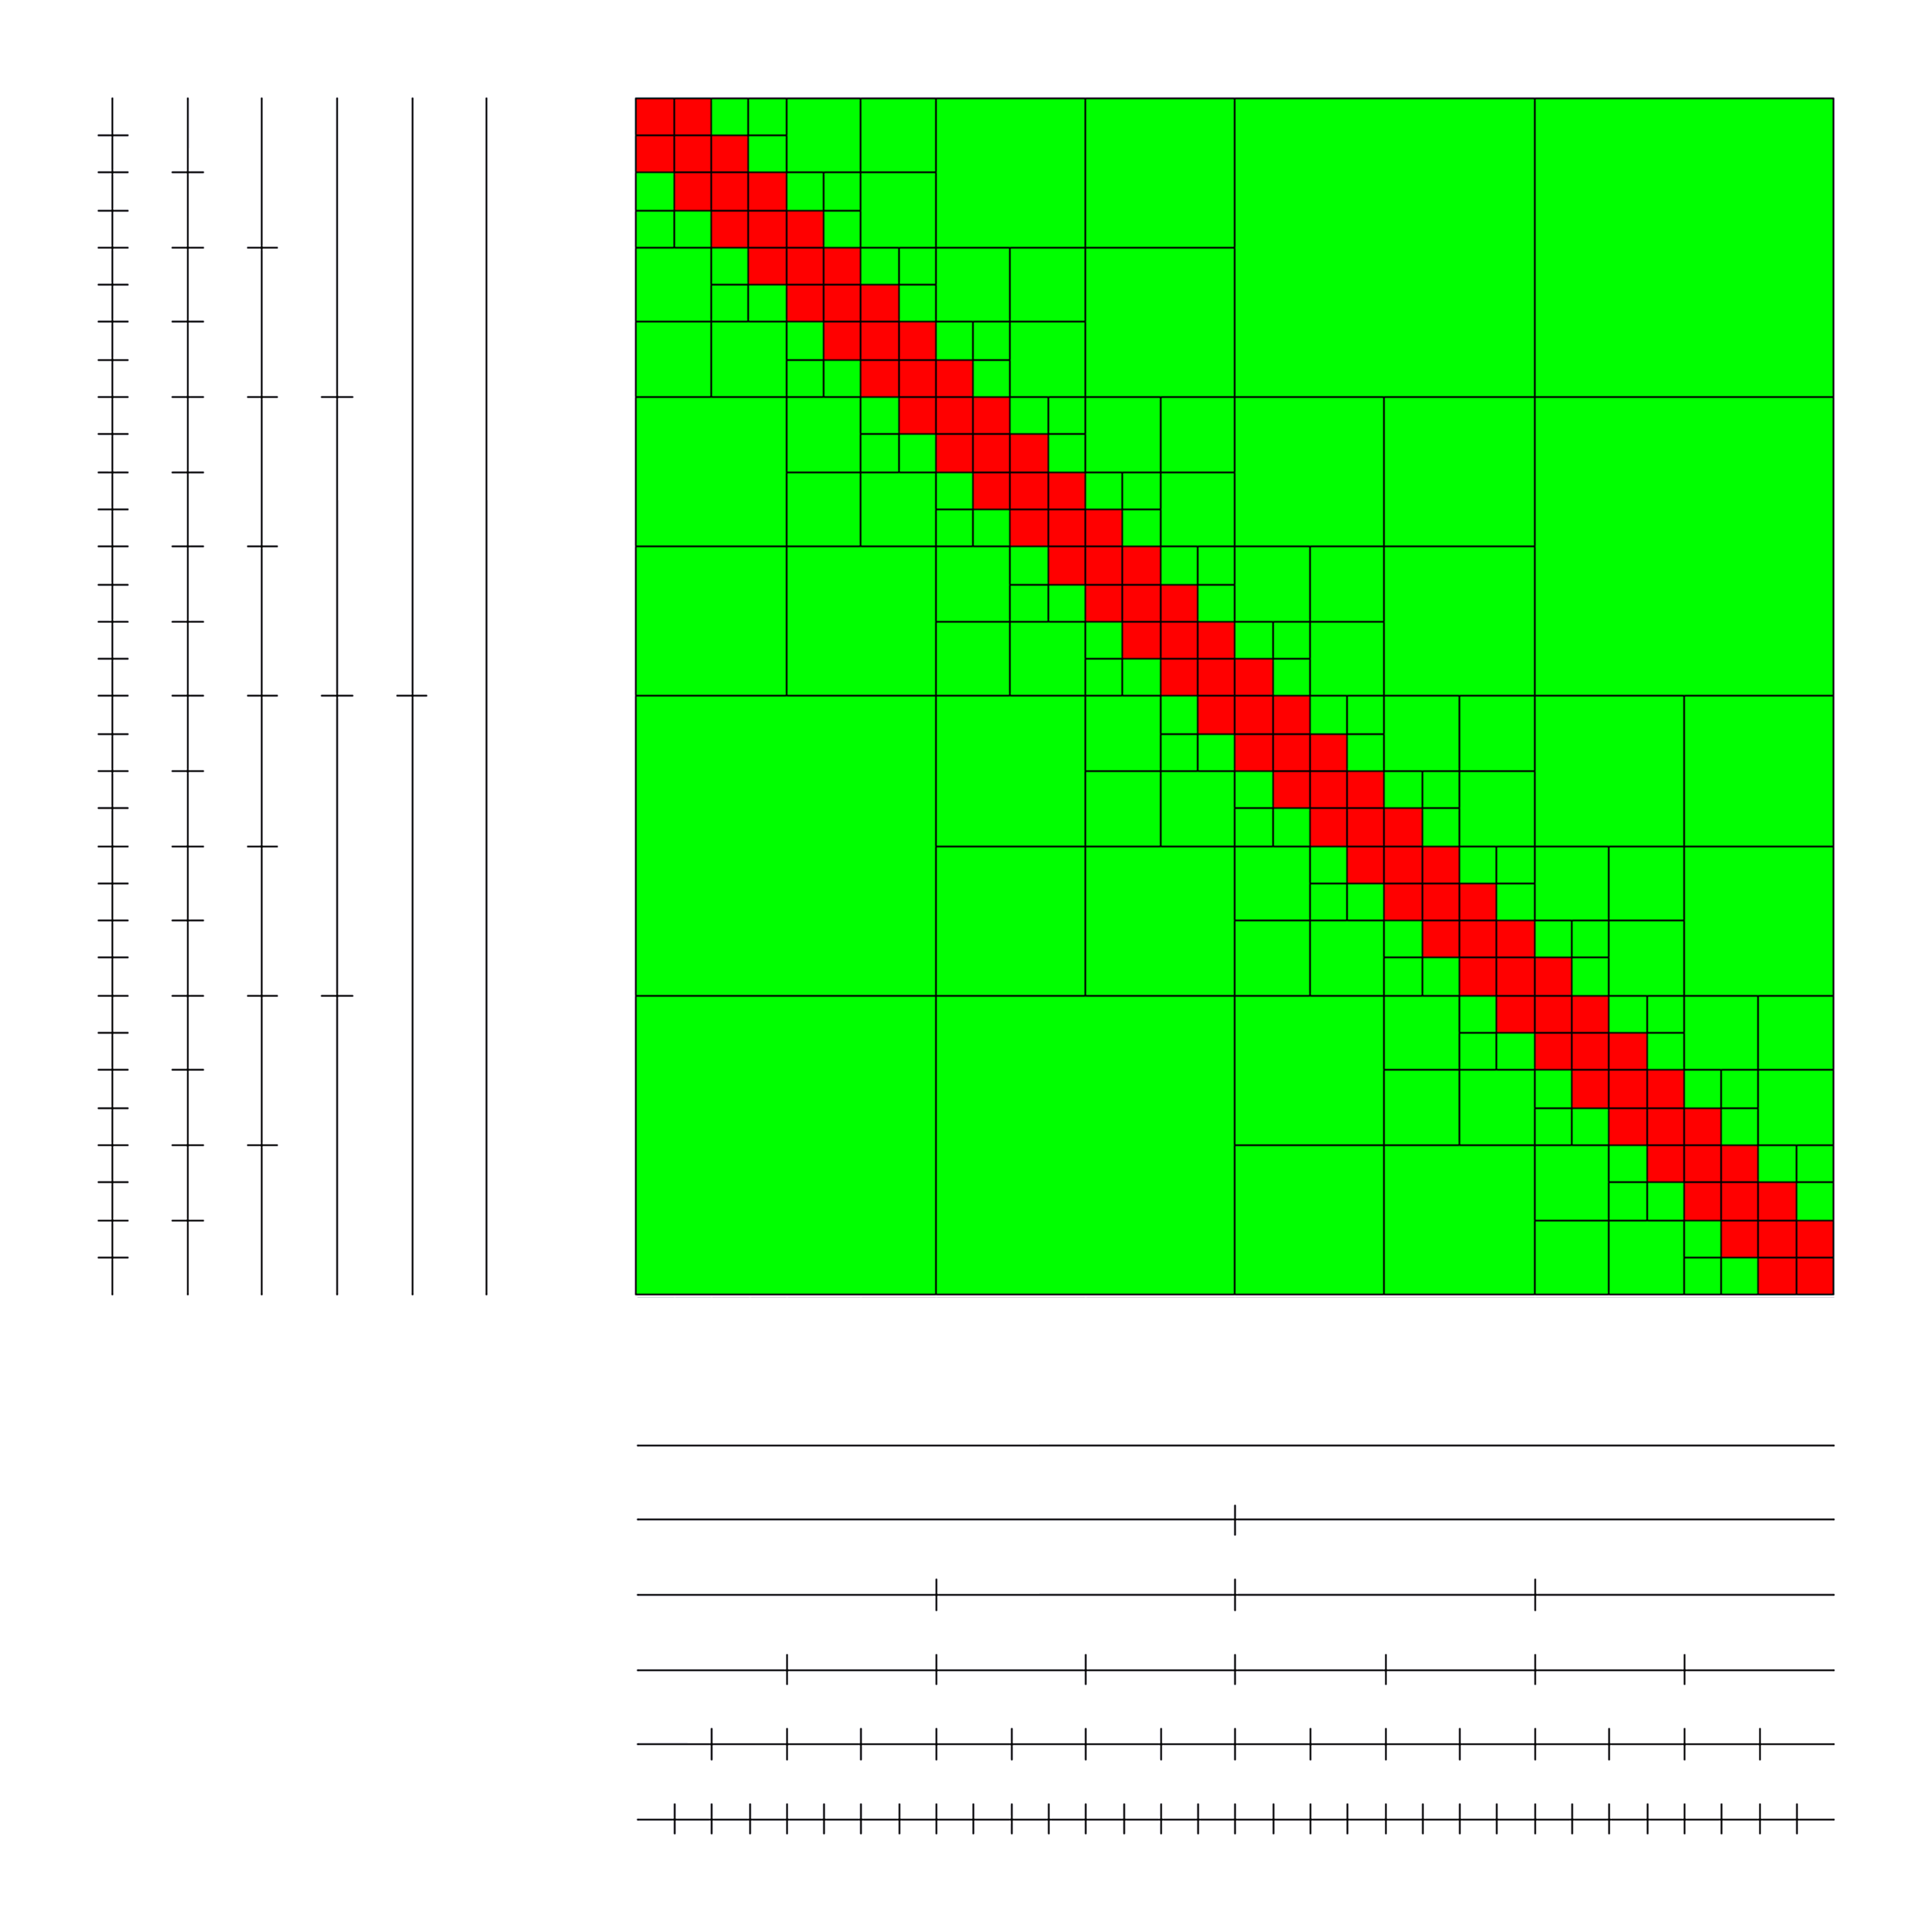
\includegraphics[width=0.68\textwidth]{img/blockbaum.png}
	\caption{Schematische Darstellung eines Blockbaumes. In grün sind zulässige, in rot unzulässige Blöcke gekennzeichnet. (Quelle: \citet{h2-slides})}
	\label{fig:blockbaum}
      \end{figure}
      
      \begin{defn}
	(Blockbaum, (streng) zulässiger Blockbaum)\\
	Seien Menge $X, Y$ und jeweils zugehörige Clusterbäume $T_X$ und $T_Y$ gegeben.
	
	Einen Clusterbaum $T_{X \times Y}$ der Menge $X \times Y$ mit folgenden Eigenschaften:
	\begin{enumerate}
	  \item Für alle Knoten $b \in T_{X \times Y}$ existieren Knoten $t \in T_X$ und $s \in T_Y$, sodass $b = t \times s$
	  \item Falls $b = t \times s \in T_{X \times Y}$ kein Blatt ist, gilt
	  \begin{equation*}
	    sons\left(b\right) = 
	    \begin{cases}
	      \{ t \times s'\ \,\ | \  s'\!\in sons\left(s\right) \} & \text{falls } sons\left(t\right) = \emptyset, \ sons\left(s\right) \neq \emptyset \\
	      \{ t' \times s\ \,\ | \  t'  \in sons\left(t\right) \} & \text{falls } sons\left(t\right) \neq \emptyset, \ sons\left(s\right) = \emptyset \\
	      \{ t' \times s' \:\ | \  t'  \in sons\left(t\right),\ s' \in sons\left(s\right) \} & \text{ansonsten}\\
	    \end{cases}
	  \end{equation*}
	\end{enumerate}
	nennen wir \textit{Blockbaum} und seine Knoten \textit{Blöcke}. Die Komponenten $t \in T_X$ und $s \in T_Y$ werden auch \textit{Zeilen-} und \textit{Spaltencluster}
	genannt.
	
	Wir nennen einen Block $b = t \times s$ \textit{zulässig} bezüglich einer Zulässigkeitsbedingung $\mathcal{Z}$, wenn $\mathcal{Z}\left(t,s\right) = \ttit{zulässig}$ erfüllt ist.
	
	Wir nennen einen Blockbaum zulässig, wenn für alle Blattblöcke $b = t \times s \in \mathcal{L}\left(T_{X \times Y}\right)$ gilt:
	\begin{equation*}
	  \mathcal{Z}\left(t,s\right) = \ttit{zulässig} \text{ oder }
	  sons\left(t\right) = \emptyset \text{ oder }
	  sons\left(s\right) = \emptyset.
	\end{equation*}      
	Wir nennen ihn \textit{streng zulässig}, wenn gilt:
	\begin{equation*}
	  \mathcal{Z}\left(t,s\right) = \ttit{zulässig} \text{ oder }
	  sons\left(t\right) = \emptyset = sons\left(s\right),
	\end{equation*}
	Mit
	\begin{align*}
		      \mathcal{L}^+\left(T_{X \times Y}\right) &= \{ b = t \times s \in  \mathcal{L}\left(T_{X \times Y}\right) \ | \ \mathcal{Z}\left(t,s\right) = \ttit{zulässig} \}\\
	  \text{und } \mathcal{L}^-\left(T_{X \times Y}\right) &= \{ b = t \times s \in  \mathcal{L}\left(T_{X \times Y}\right) \ | \ \mathcal{Z}\left(t,s\right) = \ttit{unzulässig} \}
	\end{align*}
	bezeichnen wir die Mengen der zulässigen beziehungsweise unzulässigen Blätter eines Blockbaumes. $\mathcal{L}^+\left(T_{X \times Y}\right)$ wird auch \textit{Fernfeld} und 
	$\mathcal{L}^-\left(T_{X \times Y}\right)$ \textit{Nahfeld} genannt. Die Namen leiten sich von der $\eta$-Zulässigkeitsbedingung her, die auf der relativen Nähe der Cluster zueinander beruht.
	
      \end{defn}

      
      Mit Hilfe von Blockbäumen können wir nun also Paare von Teilgebieten hierarchisch strukturieren und auf Zulässigkeit prüfen.
      In \autoref{fig:blockbaum} ist ein Blockbaum, beziehungsweise die Blätter eines Blockbaumes, dargestellt. Zulässige Blattblöcke sind grün, unzulässige rot gekennzeichnet. Zur linken
      den Blockbaumes ist der Clusterbaum mit den Targetclustern, unten der Clusterbaum mit den Sourceclustern schematisch abgebildet.
%       Damit haben wir nun alles Notwendige bei der Hand um \hmat definieren zu können.
      
  \subsection{\hmat}
  \label{sec:hmat}
    \begin{defn}
      (\Rk-Matrix)\\
      Seien $m,n,k \in \N$ sowie $M \in \R^{m \times n}$ gegeben. Wir nennen $M$ eine \textit{\Rk-Matrix}, wenn Matrizen $A \in \R^{m \times k}$ und $B \in \R^{n \times k}$  existieren, sodass
      \begin{equation*}
	M = A \trans{B}
      \end{equation*}
      gilt. Die Menge aller solcher \Rk-Matrizen bezeichnen wir mit
      \begin{equation*}
	\mathcal{R}\left(m,n,k\right) = \{M \in \R^{m \times n} \ | \ M = A\trans{B}, A \in \R^{m \times k}, B \in \R^{n \times k}\}.
      \end{equation*}
      \citep{nichtlokop}
    \end{defn}
    
    Das praktische an \Rk-Matrizen ist, dass sie sich durch $k\left(m+n\right)$ Koeffizienten darstellen lassen. Ist $k \ll m,n$ ist dies wesentlich effizienter als eine volle Darstellung mit $m \cdot n$ 
    Koeffizienten. \citep{nichtlokop}
    
    \begin{defn}
    \label{def:hmat}
      (Hierarchische Matrix oder $\mathcal{H}$-Matrix)\\
      Seien $X$, $Y$ zwei Mengen, $T$ ein zugehöriger zulässiger Blockbaum mit Zulässigkeitsbedingung $\mathcal{Z}$ und $k: \mathcal{L}\left(T\right) \to \N_0$ die Rangverteilung der Blätter.
      
      Eine Matrix $M \in \R^{X \times Y}$ heißt \textit{hierarchische Matrix} oder kurz \textit{$\mathcal{H}$-Matrix} bezüglich $T$, $\mathcal{Z}$ und $k$, falls für jeden Blattblock
      $b \in \mathcal{L}\left(T\right)$ der korrespondierende Matrixblock $M_b = \left(M_{ij}\right)_{\left(i,j\right) \in b}$ eine \Rk-Matrix ist.
      
      Eine Zahl $k_0 \in \N$ mit $k\left(b\right) \leq k_0$ für alle $b \in \mathcal{L}^+\left(T_{X \times Y}\right)$ heißt lokaler Rang der hierarchischen Matrix.
      
      \citep{h2diss, nichtlokop}
      
    \end{defn}
    
    \begin{figure}[t]
      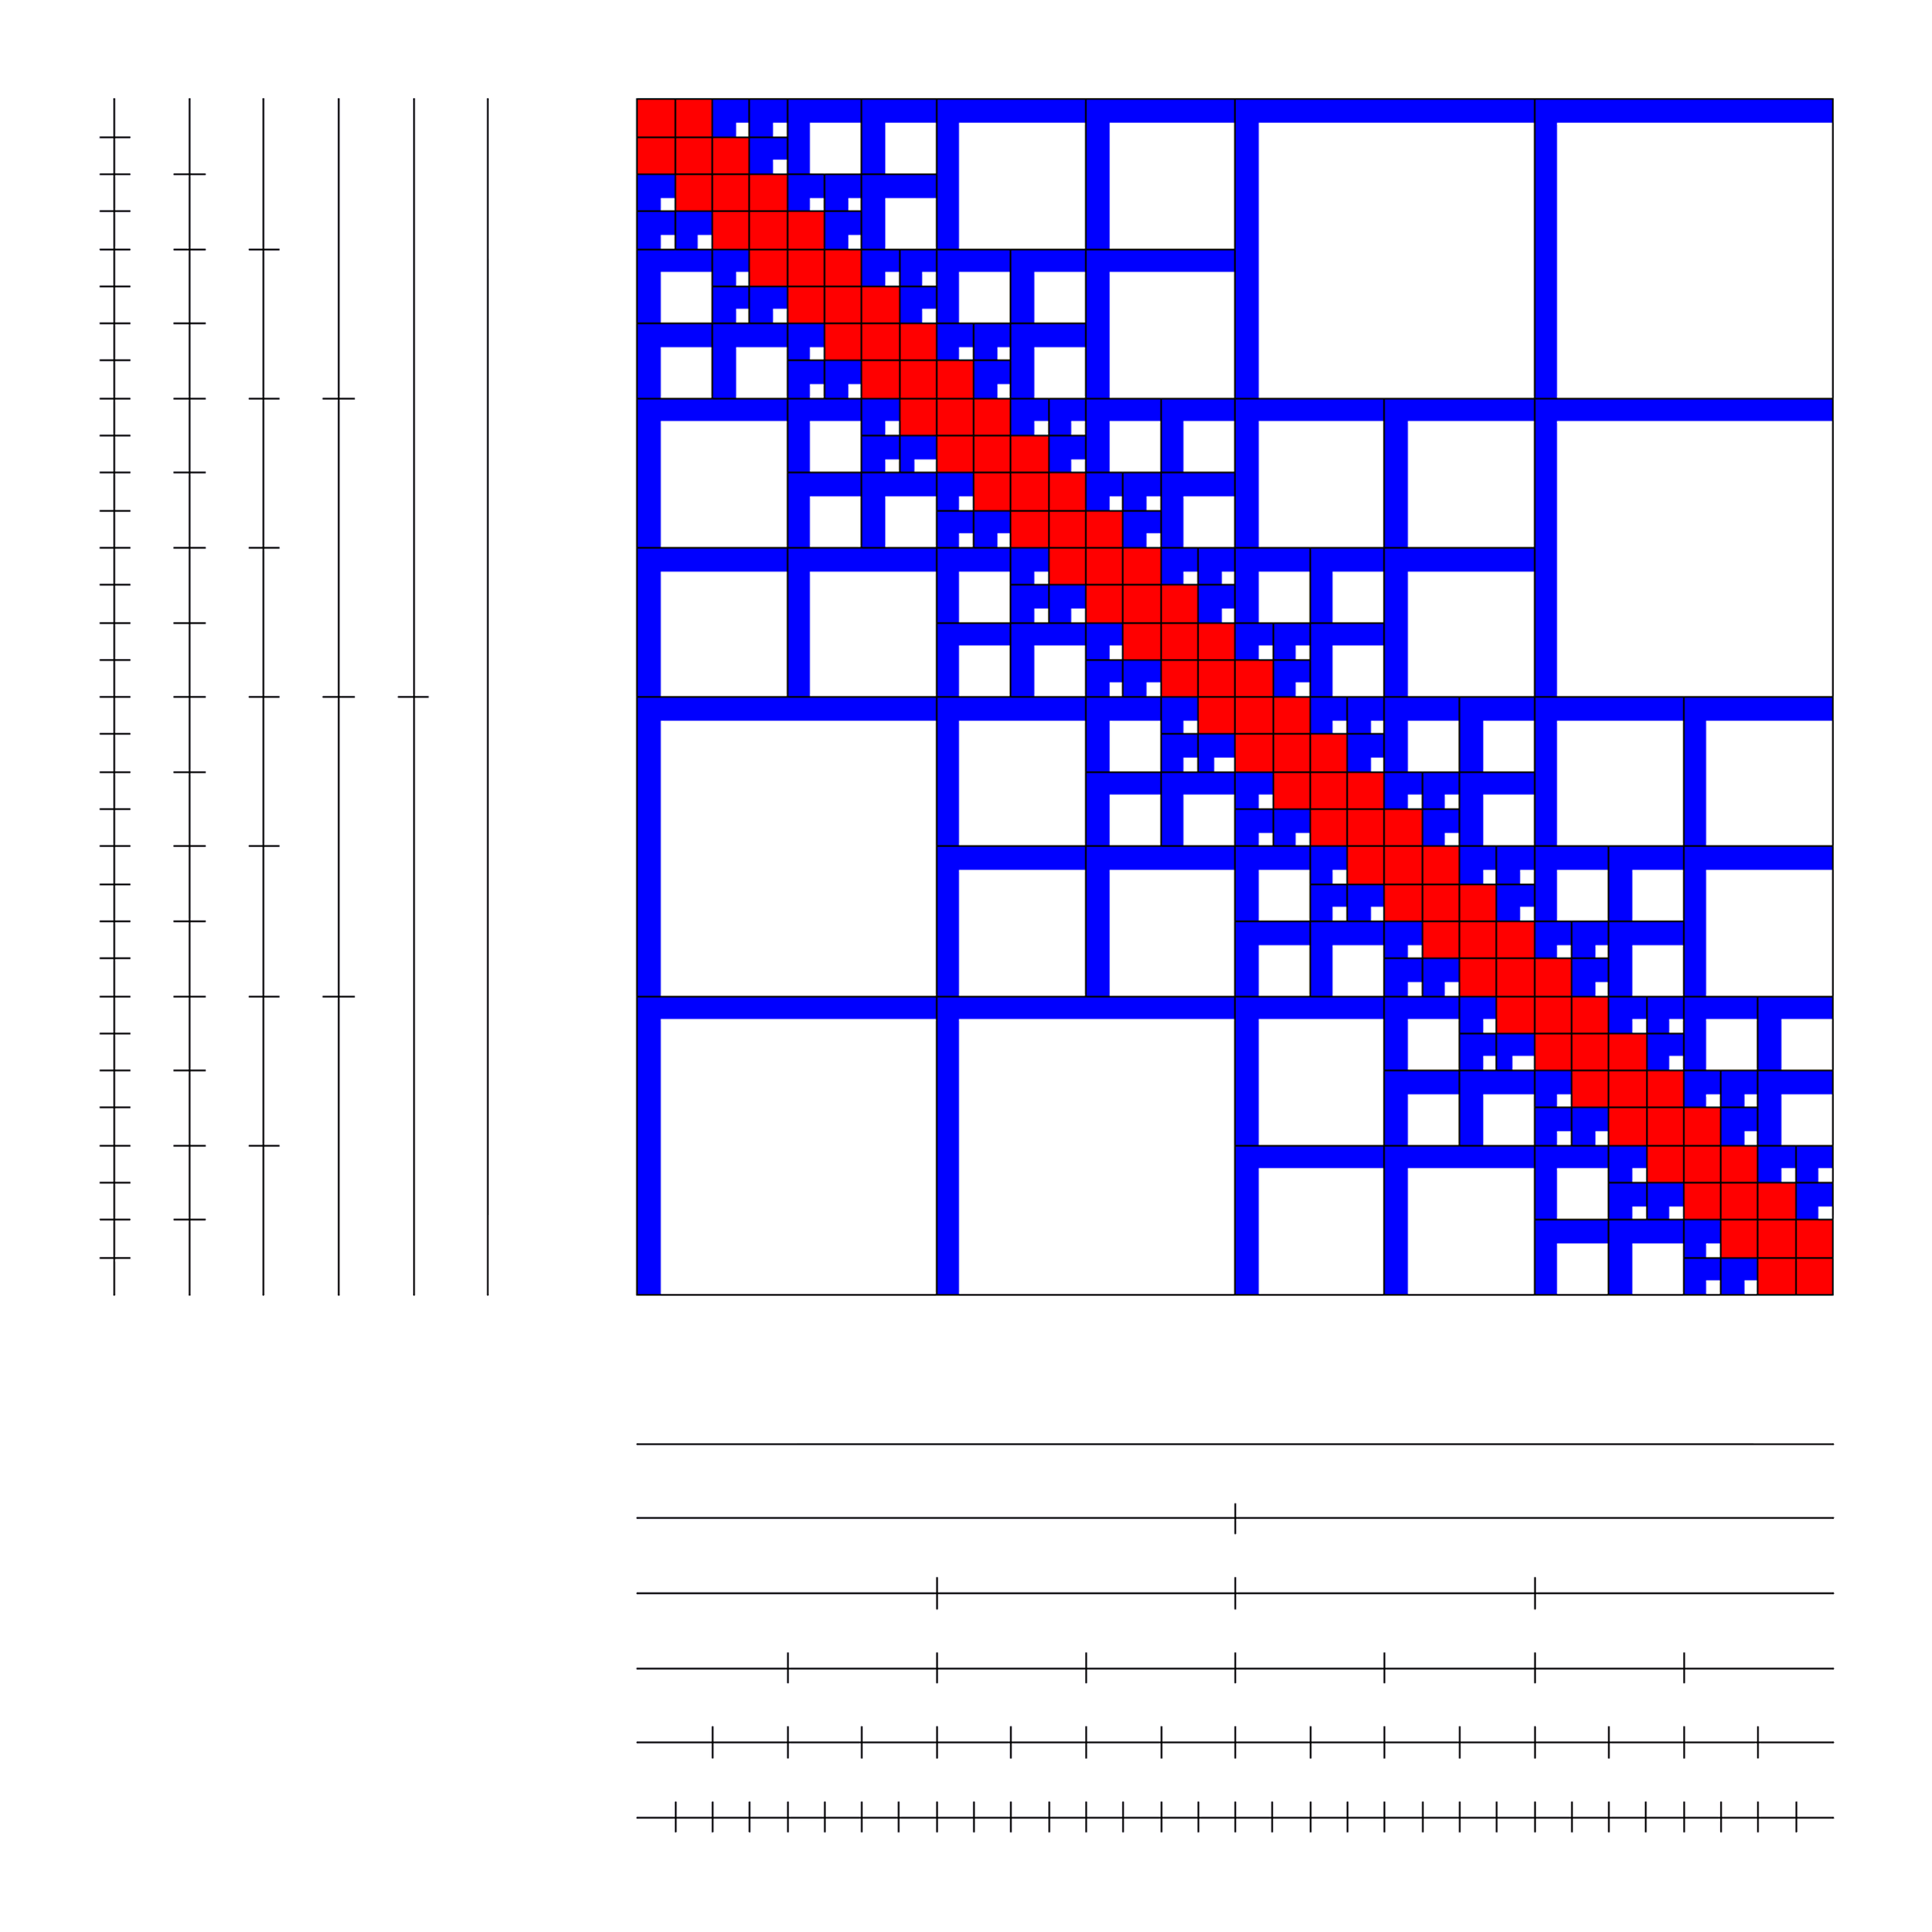
\includegraphics[width=0.7\textwidth]{img/h-matrix.png}
      \caption{Schematische Darstellung einer $\mathcal{H}$-Matrix. In blau sind die Matrizen $A_b$ und $B_b$, in rot die Matrizen $N_b$ gekennzeichnet. (Quelle: \citet{h2slides})}
      \label{fig:hmat}
    \end{figure}


    Für die Darstellung in Computern sind \hmat von besonderem Interesse, da sie sich durch die Zerlegung in \Rk-Matrizen besonders kompakt speichern lassen. Für eine $\mathcal{H}$-Matrix
    $M$ mit lokalem Rang $k$ existieren nach Definition Familien von Matrizen $\left(A_b\right)_{b \in \mathcal{L}^+\left(T_{X \times Y}\right)} \text{ und } \left(B_b\right)_{b \in \mathcal{L}^+\left(T_{X \times Y}\right)}$, mit 
    \begin{equation*}
      A_b \in \R^{t \times k}, B_b \in \R^{s \times k}, \left. M \right|_b = A_b\trans{B_b} \text{, für alle } b = t \times s \in \mathcal{L}^+\left(T_{X \times Y}\right).
    \end{equation*}
    So verbleiben nur noch für unzulässige Blöcke $b \in \mathcal{L}^-\left(T_{X \times Y}\right)$ vollbesetzte Matrizen $N_b = M|_b$, sogenannte \textit{Nahfeldmatrizen}.
    Das Tripel $\left( \left(A_b\right)_{b \in \mathcal{L}^+\left(T_{X \times Y}\right)} , \left(B_b\right)_{b \in \mathcal{L}^+\left(T_{X \times Y}\right)} , \left(N_b\right)_{b \in \mathcal{L}^-\left(T_{X \times Y}\right)} \right)$ bezeichnen wir als $\mathcal{H}$-
    Matrix-Darstellung der Matrix $M$. \citep{nichtlokop} 
    
    In \autoref{fig:hmat} ist eine $\mathcal{H}$-Matrix schematisch dargestellt. Für zulässige Blöcke sind die Matrizen $A_b$ und $B_b$ in blau 
    und die Nahfeldmatrizen $N_b$ in rot gekennzeichnet. Durch die Dicke der Matrizen $A_b$ und $B_b$ ist der lokale Rang $k$ dargestellt. die Speicherplatzersparnis ist dadurch gut zu erkennen.
    
    Gerade auch im Zusammenhang mit dieser Arbeit ist aber von noch größerem Interesse, dass auch Operationen wie Matrix-Vektor-Multiplikationen auf \Rk-Matrizen und damit auch auf \hmat wesentlich 
    effektiver implementiert werden können. \citet{h2diss} zeigt, dass die Matrix-Vektor-Multiplikation nur $k\left(n+m\right)$ statt $n \cdot m$ Operationen benötigt.
    
%     \clearpage
    
    \subsection{Optimierung}
    \label{sec:optimierung}
    Im Folgenden wollen wir noch einige Überlegungen vorstellen, durch die \hmat noch speicherplatzsparender und noch effizienter in der Berechnung werden.
    
    \subsubsection{Zeilen- und Spaltenmatrizen}
    
    \begin{figure}[b]
      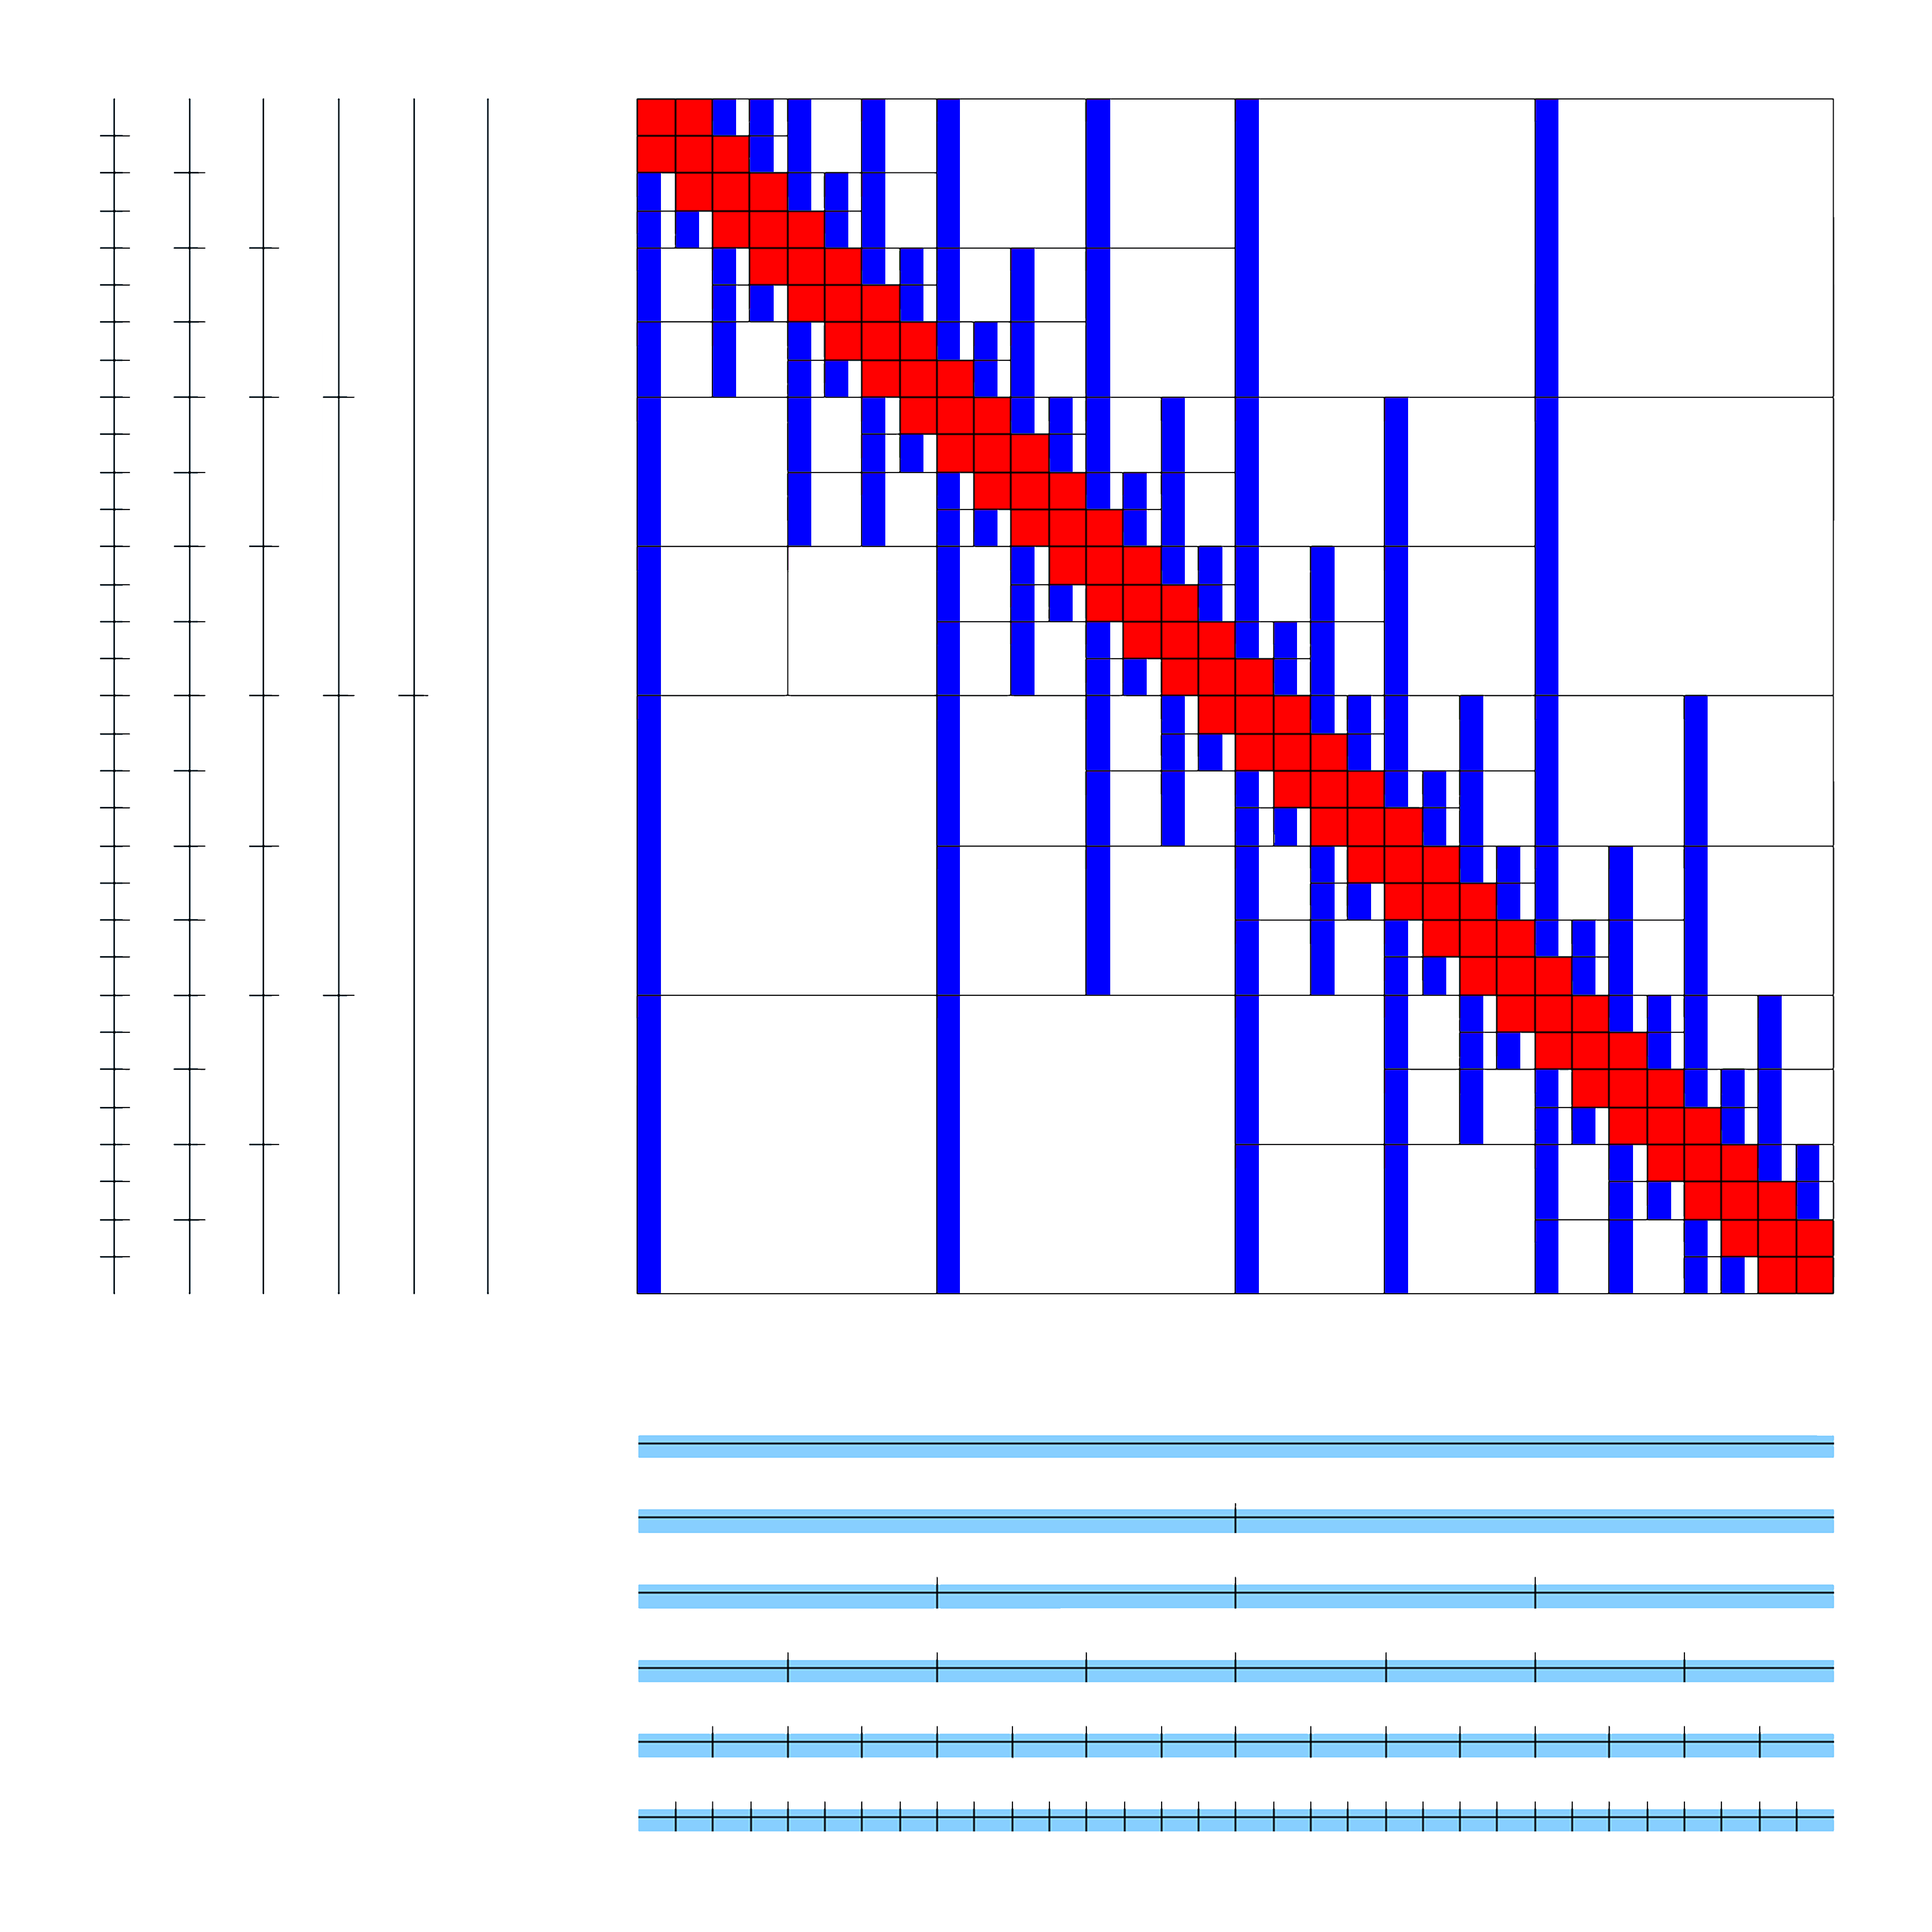
\includegraphics[width=0.7\textwidth]{img/semi-h2-matrix.png}
      \caption{Darstellung der Ersetzung der Matrizen $B_b$ durch Spaltenmatrizen $W_\sigma$. Letztere sind in hellblau auf dem Clusterbaum eingezeichnet. Die verbleibenden dunkelblauen 
	       Matrizen sind die Matrizen $A_b$. (Quelle: \citet{h2slides})}
      \label{fig:semi-h2}
    \end{figure}
    
    Bisher wurde eine hierarchische Matrix konstruiert, indem die Kernfunktion $g$ auf zulässigen Blöcken $b = \tau \times \sigma \in \mathcal{L}^+\left(T_{X \times Y}\right)$ durch die auf $\sigma$ 
    interpolierte Funktion
    \begin{equation*}
      g_\sigma\left(x, y\right) = \sum_{\nu \in \haken{k}} g\left(x, \xi_\inds{\nu}\right) \lag_\inds{\nu}\left(y\right)
    \end{equation*}
    approximiert wurde. Somit erhalten wir durch die punktweise Definition
    \begin{equation*}
      \left(A_b\right)_{x\nu} := g\left(x, \xi_\inds{\nu}\right) \text{ und } \left(B_b\right)_{y\nu} := \lag_\inds{\nu}\left(y\right) \text{ für alle } x \in \tau \text{ und } y \in \sigma
    \end{equation*}
    Matrizen $A_b \in \R^{m \times k}$ und $B_b \in \R^{n \times k}$. Damit können wir die Matrix $G$ auf Blöcken $b \in \mathcal{L}^+\left(T_{X \times Y}\right)$ in der Form 
    \begin{equation*}
      \left(G|_b\right)_{xy} = g\left(x,y\right) \approx g_\sigma\left(x,y\right) = \left(A_b \trans{B_b}\right)_{xy},
    \end{equation*}
    also durch \Rk-Matrizen darstellen und erhalten so eine Darstellung als hierarchische Matrix. \citep{nichtlokop}
    
    Ein Blick auf die Definition der Matrix $B_b$ verrät, dass diese nicht von $\tau$ sondern ausschließlich von $\sigma$ abhängt. Wir können sie also für konstantes $\sigma$ für alle Blöcke 
    $\tilde b = \tilde \tau \times \sigma \in T_{X \times Y}$ durch eine Matrix
    \begin{equation*}
      \left(W_\sigma\right)_{y\nu} := \lag_\inds{\nu}\left(y\right)
    \end{equation*} 
    ersetzen. Anstatt also für jeden Block $b$ wieder eine eigene Matrix aufstellen zu müssen, können sich Blöcke mit gleichem Quellgebiet $\sigma$ die Matrizen teilen. Insbesondere muss diese 
    Matrix $W_\sigma$ auch nur einmal berechnet werden, womit ein erheblicher Teil des Rechnungsaufwands bei der Konstruktion von \hmat eingespart werden kann. Zudem können wiederum Operationen
    wie die Matrix-Vektor-Multiplikation effektiver durchgeführt werden, da auch hier die Matrix $W_\sigma$ ausgeklammert werden kann, und so nur einmal in die Berechnung einfließt. \citep{nichtlokop}
    
    \begin{defn}
      (Zeilen-/Spaltenmatrizen)\\
      Wir nennen Matrizen $W_\sigma \in \R^{\sigma \times k}$ wie oben \textit{Spaltenmatrizen} einer hierarchischen Matrix $G$. Bei Interpolation in der ersten Komponente nennen wir sie 
      entsprechend \textit{Zeilenmatrizen}.
    \end{defn}

    Dargestellt ist diese Optimierung in \autoref{fig:semi-h2}. In hellblau wurden die Spaltenmatrizen $W_\sigma$ auf dem Clusterbaum eingezeichnet. Die verbleibenden dunkelblauen Matrizen sind
    die nicht optimierten Matrizen $A_b$. Ein Vergleich der Häufigkeit der Matrizen $A_b$ und $W_\sigma$ verdeutlicht die zuvor beschriebene Ersparnis von Redundanz.

    
    \subsubsection{Transfermatrizen und Clusterbasis}
    \label{sec:transmat}
    Von \citet{h2approxint} wird auf folgende Eigenschaft der Interpolationsoperatoren hingewiesen:

    Sei $\mathcal{Q}_k := \{ \prod_{i \in \haken{i_0}} p_i \ | \ p_i \in \Pi_k , \ i_0 \in \N \}$ der durch Tensorprodukte von Polynomen von höchstens Grad $k$ aufgespannte Polynomraum.
    Da alle Cluster durch Polynome der selben Ordnung interpoliert wurden, zeigt \autoref{eq:interpol}, dass $\mathfrak{I}_Q$ gerade eine Projektion auf diesen Raum $\mathcal{Q}_k$ ist.
    
    Wegen dieser Projektionseigenschaft des Interpolationsoperators folg für $\sigma \in T_X \backslash \mathcal{L}\left(T_X\right)$, Söhne $\tilde \sigma \in sons\left(\sigma\right)$ und 
    für alle $\nu \in \haken{k}$:
    \begin{equation*}
      \lag_\inds{\nu} = \mathfrak{I}_{\tilde \sigma}[\lag_\inds{\nu}] = \sum_{\tilde \nu \in \haken{k}} \lag_\inds{\nu}\left(\xi_{\tilde \sigma,\tilde \nu}\right) \lag_{\tilde \sigma,\tilde \nu}.
    \end{equation*}
    
    Anstatt also auf jeder Ebene des Clusterbaumes eine vollständige Matrix $W_\sigma \in \R^{\sigma \times k}$ aufzustellen, genügt es für jeden Sohncluster $\tilde \sigma \in sons\left(\sigma\right)$
    Matrizen $E_{\tilde \sigma} \in \R^{k \times k}$ mit $\left(E_{\tilde \sigma}\right)_{\tilde\nu , \nu} := \lag_\inds{\nu}\left(\xi_{\tilde \sigma, \tilde \nu}\right)$ zu speichern. Dies führt zu 
    folgender Definition:
    
    \begin{defn}
      (Transfermatrix, Clusterbasis)\\
      Sei $T_X$ ein Clusterbaum mit einer Familie von Spalten- (bzw. Zeilen-)matrizen $W = \left(W_\sigma\right)_{\sigma \in T_X}$. Existiert eine Familie $E = \left(E_\sigma\right)_{\sigma \in T_X}$ 
      von $\left(k \times k\right)$-Matrizen mit der Eigenschaft
      \begin{equation*}
	\left. V_\sigma \right|_{\tilde \sigma \times k} = V_{\tilde \sigma} E_{\tilde \sigma} \ \ \ \ \ \ \ \ \ \ \ \ \text{für alle } 
	\sigma \in T_X \backslash \mathcal{L}\left(T_X\right) \text{ und } \tilde \sigma \in sons\left(\sigma\right),
      \end{equation*}
      so nennen wir $V$ eine \textit{(geschachtelte) Clusterbasis} (von Rang $k$) für den Clusterbaum $T_X$. Die Matrizen der Familie $E$ heißen die korrespondierenden \textit{Transfermatrizen}.
      \citep{nichtlokop}
    \end{defn}

    Mit der \textit{geschachtelten Darstellung} $\left(\left(W_\sigma\right)_{\sigma in \mathcal{L}\left(T_X\right)} , \left(E_\sigma\right)_{\sigma \in T_X \backslash \mathcal{L}\left(T_X\right)}\right)$ der Clusterbasen haben wir nun also eine 
    noch kompaktere Darstellung der Matrizen $B_b$. Dargestellt ist dies in \autoref{fig:trans}.
    
    \begin{figure}[t]
      \begin{tabular}{c}
	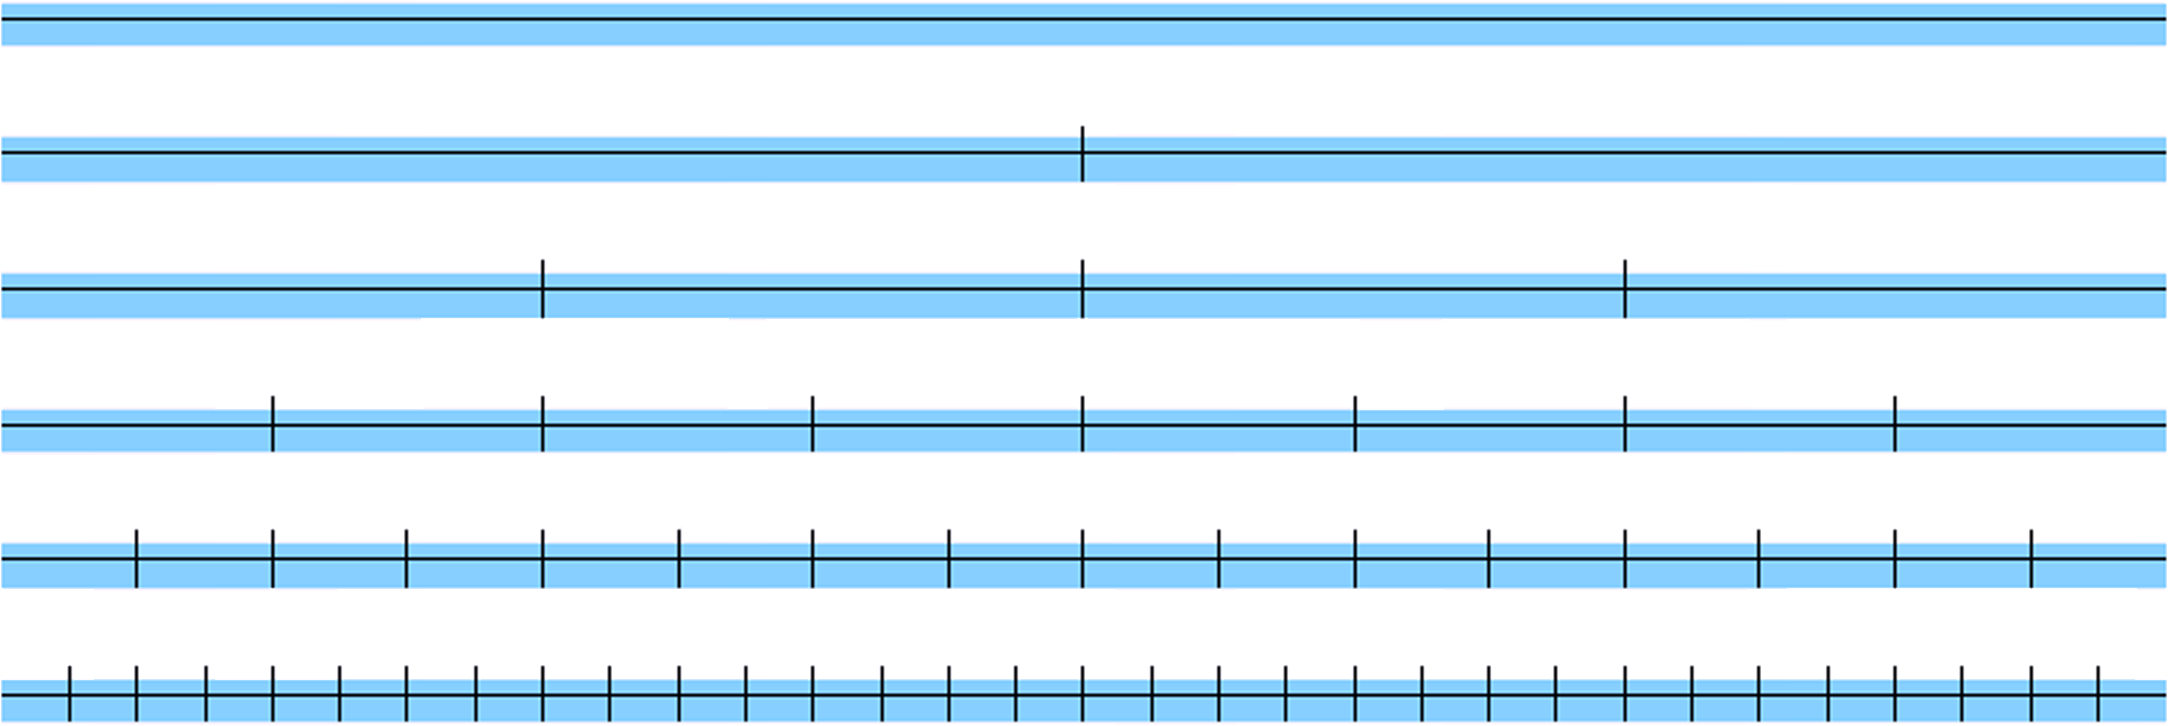
\includegraphics{img/cbaum_full.png}\\
	
	\begin{turn}{-90} $\longrightarrow$ \ \ \  \end{turn}\\
	
	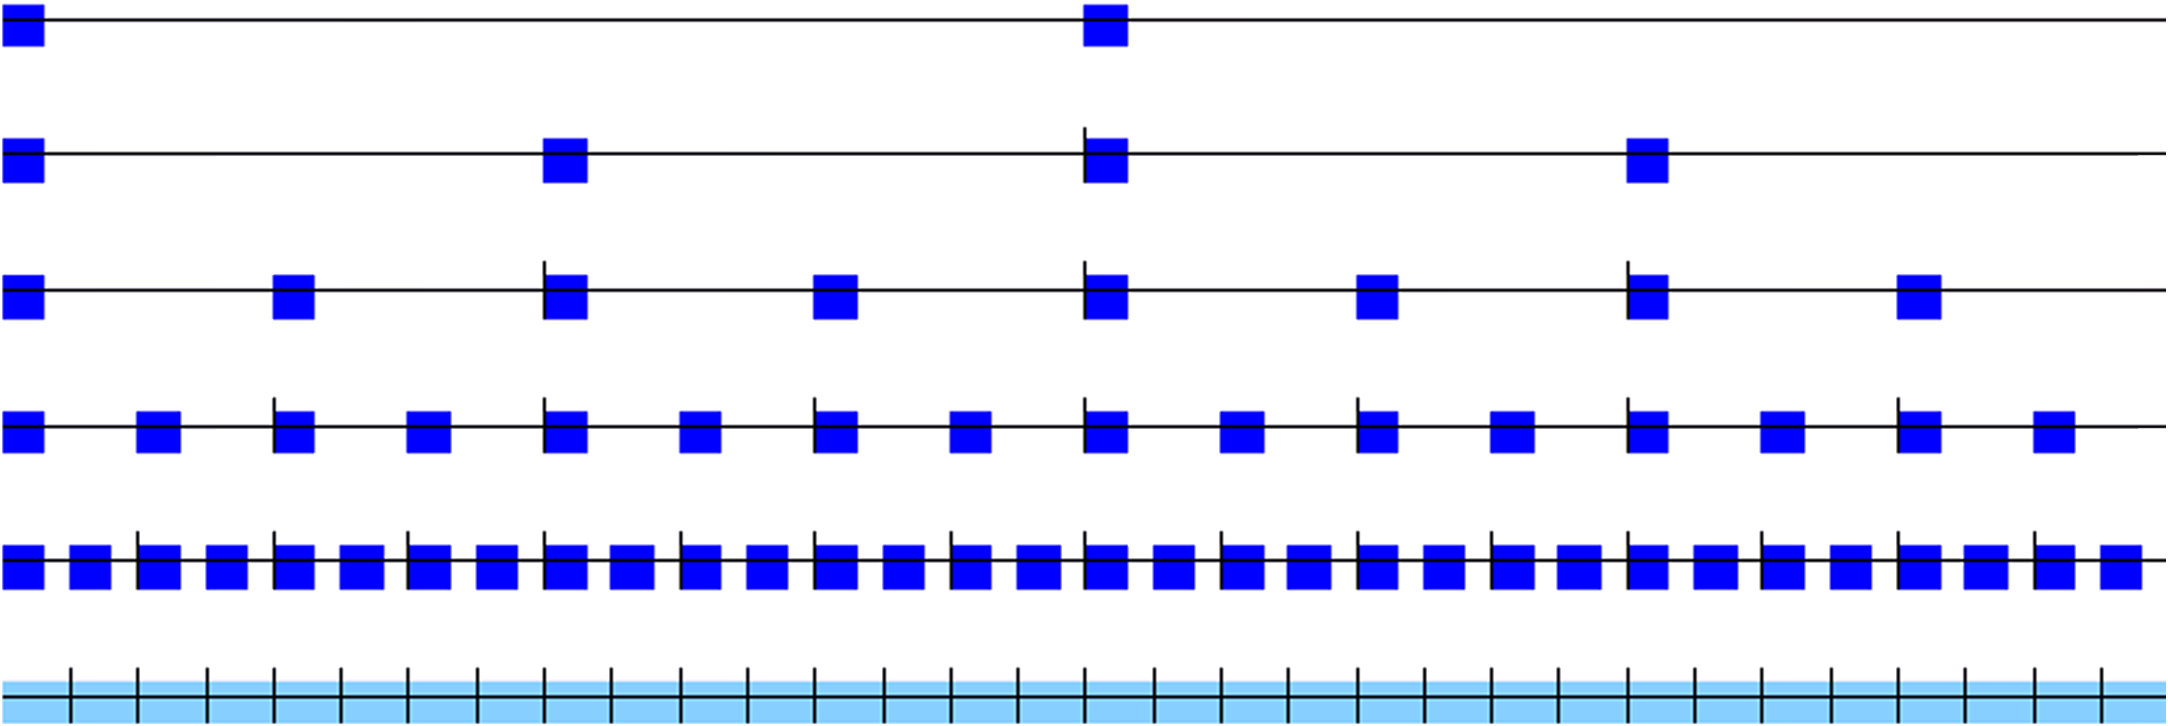
\includegraphics{img/cbaum_transfer.png}
      \end{tabular}
      \caption{Ersetzung der Matrizen $W_\sigma$ durch Transfermatrizen $E_{\tilde \sigma}$ auf Nicht-Blattclustern. (Quelle: \citet{h2slides})}
      \label{fig:trans}
    \end{figure}

    \subsubsection{Interpolation in beiden Komponenten}
    Auch in diesem Abschnitt folge ich dem Aufbau von \citet{nichtlokop}.
    
    Wir haben bereits einige Eigenschaften der Matrizen $B_b$ beziehungsweise $W_\sigma$ identifiziert, die sich zur Effektivitätssteigerung nutzen lassen.
    Leider bleiben die Speicherplatzineffizienz und der höhere Rechenaufwand für die Matrizen $A_b$ bestehen, die die positiven Eigenschaften der Matrizen $W_\sigma$ nicht teilen. Allerdings 
    haben wir die Matrizen $W_\sigma$ einfach punktweise aus den Lagrange-Polynomen bei der Interpolation definiert. Es liegt also nahe eine Interpolation nicht nur in einer, sondern in beiden 
    Variablen durchzuführen. Wir wählen also Interpolationspunkte $\xi_\indt{1}, \dots , \xi_\indt{k}$ und erhalten wiederum mit den zugehörigen Lagrange-Polynomen 
    $\lag_\indt{1}, \dots, \lag_\indt{k}$:
    \begin{equation*}
      g\left(x,y\right) \approx \tilde g\left(x,y\right) = \sum_{\mu \in \haken{k}} \sum_{\nu \in \haken{k}} \lag_\indt{\mu}\left(x\right) g\left(\xi_\indt{\mu}, \xi_\inds{\nu}\right) \lag_\inds{\nu}\left(y\right).
    \end{equation*}
    Mit 
    \begin{equation*}
      \left(S_b\right)_{\mu\nu} := g\left(\xi_\indt{\mu}, \xi_\inds{\nu}\right), \ \mu,\nu \in \haken{k}
    \end{equation*}
    erhalten wir eine Familie von Koeffizientenmatrizen $\left(S_b\right)_{b \in \mathcal{L}^+\left(T_{X \times Y}\right)} \in \R^{k \times k}$, die weder von $x$, noch von $y$ anhängt, sondern lediglich von den 
    Interpolationspunkten.
    Außerdem haben wir durch die neuerliche Interpolation die Abhängigkeit von $x$ wiederum auf Lagrange-Polynome beschränkt und erhalten so Matrizen $V_\tau \in \R^{\tau \times k}$ durch
    die Festlegung
    \begin{equation*}
      \left(V_\tau\right)_{x\mu} := \lag_\indt{\mu}\left(x\right).
    \end{equation*}
    Insgesamt erhalten wir also für alle $b = \tau \times \sigma \in \mathcal{L}^+\left(T_{X \times Y}\right)$
    \begin{equation*}
      \left. G \right|_b \approx \left. \tilde G \right|_b = V_\tau S_b \trans{W_\sigma}.
    \end{equation*}
    
    Die Matrizen $V_\tau$ haben dieselben Eigenschaften wie die Matrizen $W_\sigma$. Beide lassen sich also nicht nur effizient speichern, sondern auch effizient konstruieren. Außerdem 
    brauchen sie auf Grund der Entkoppelung von $\tau$ und $\sigma$ jeweils nur einmal aufgestellt zu werden. Da die Matrizen $S_b$, die die Kopplung zwischen den Clustern 
    $\tau$ und $\sigma$ beschreiben, wiederum verhältnismäßig klein sind, lassen sich diese wiederum auch effektiv verarbeiten.
    
    \subsection{\hquad}
    \label{sec:hquad}
    
    \begin{figure}[b]
      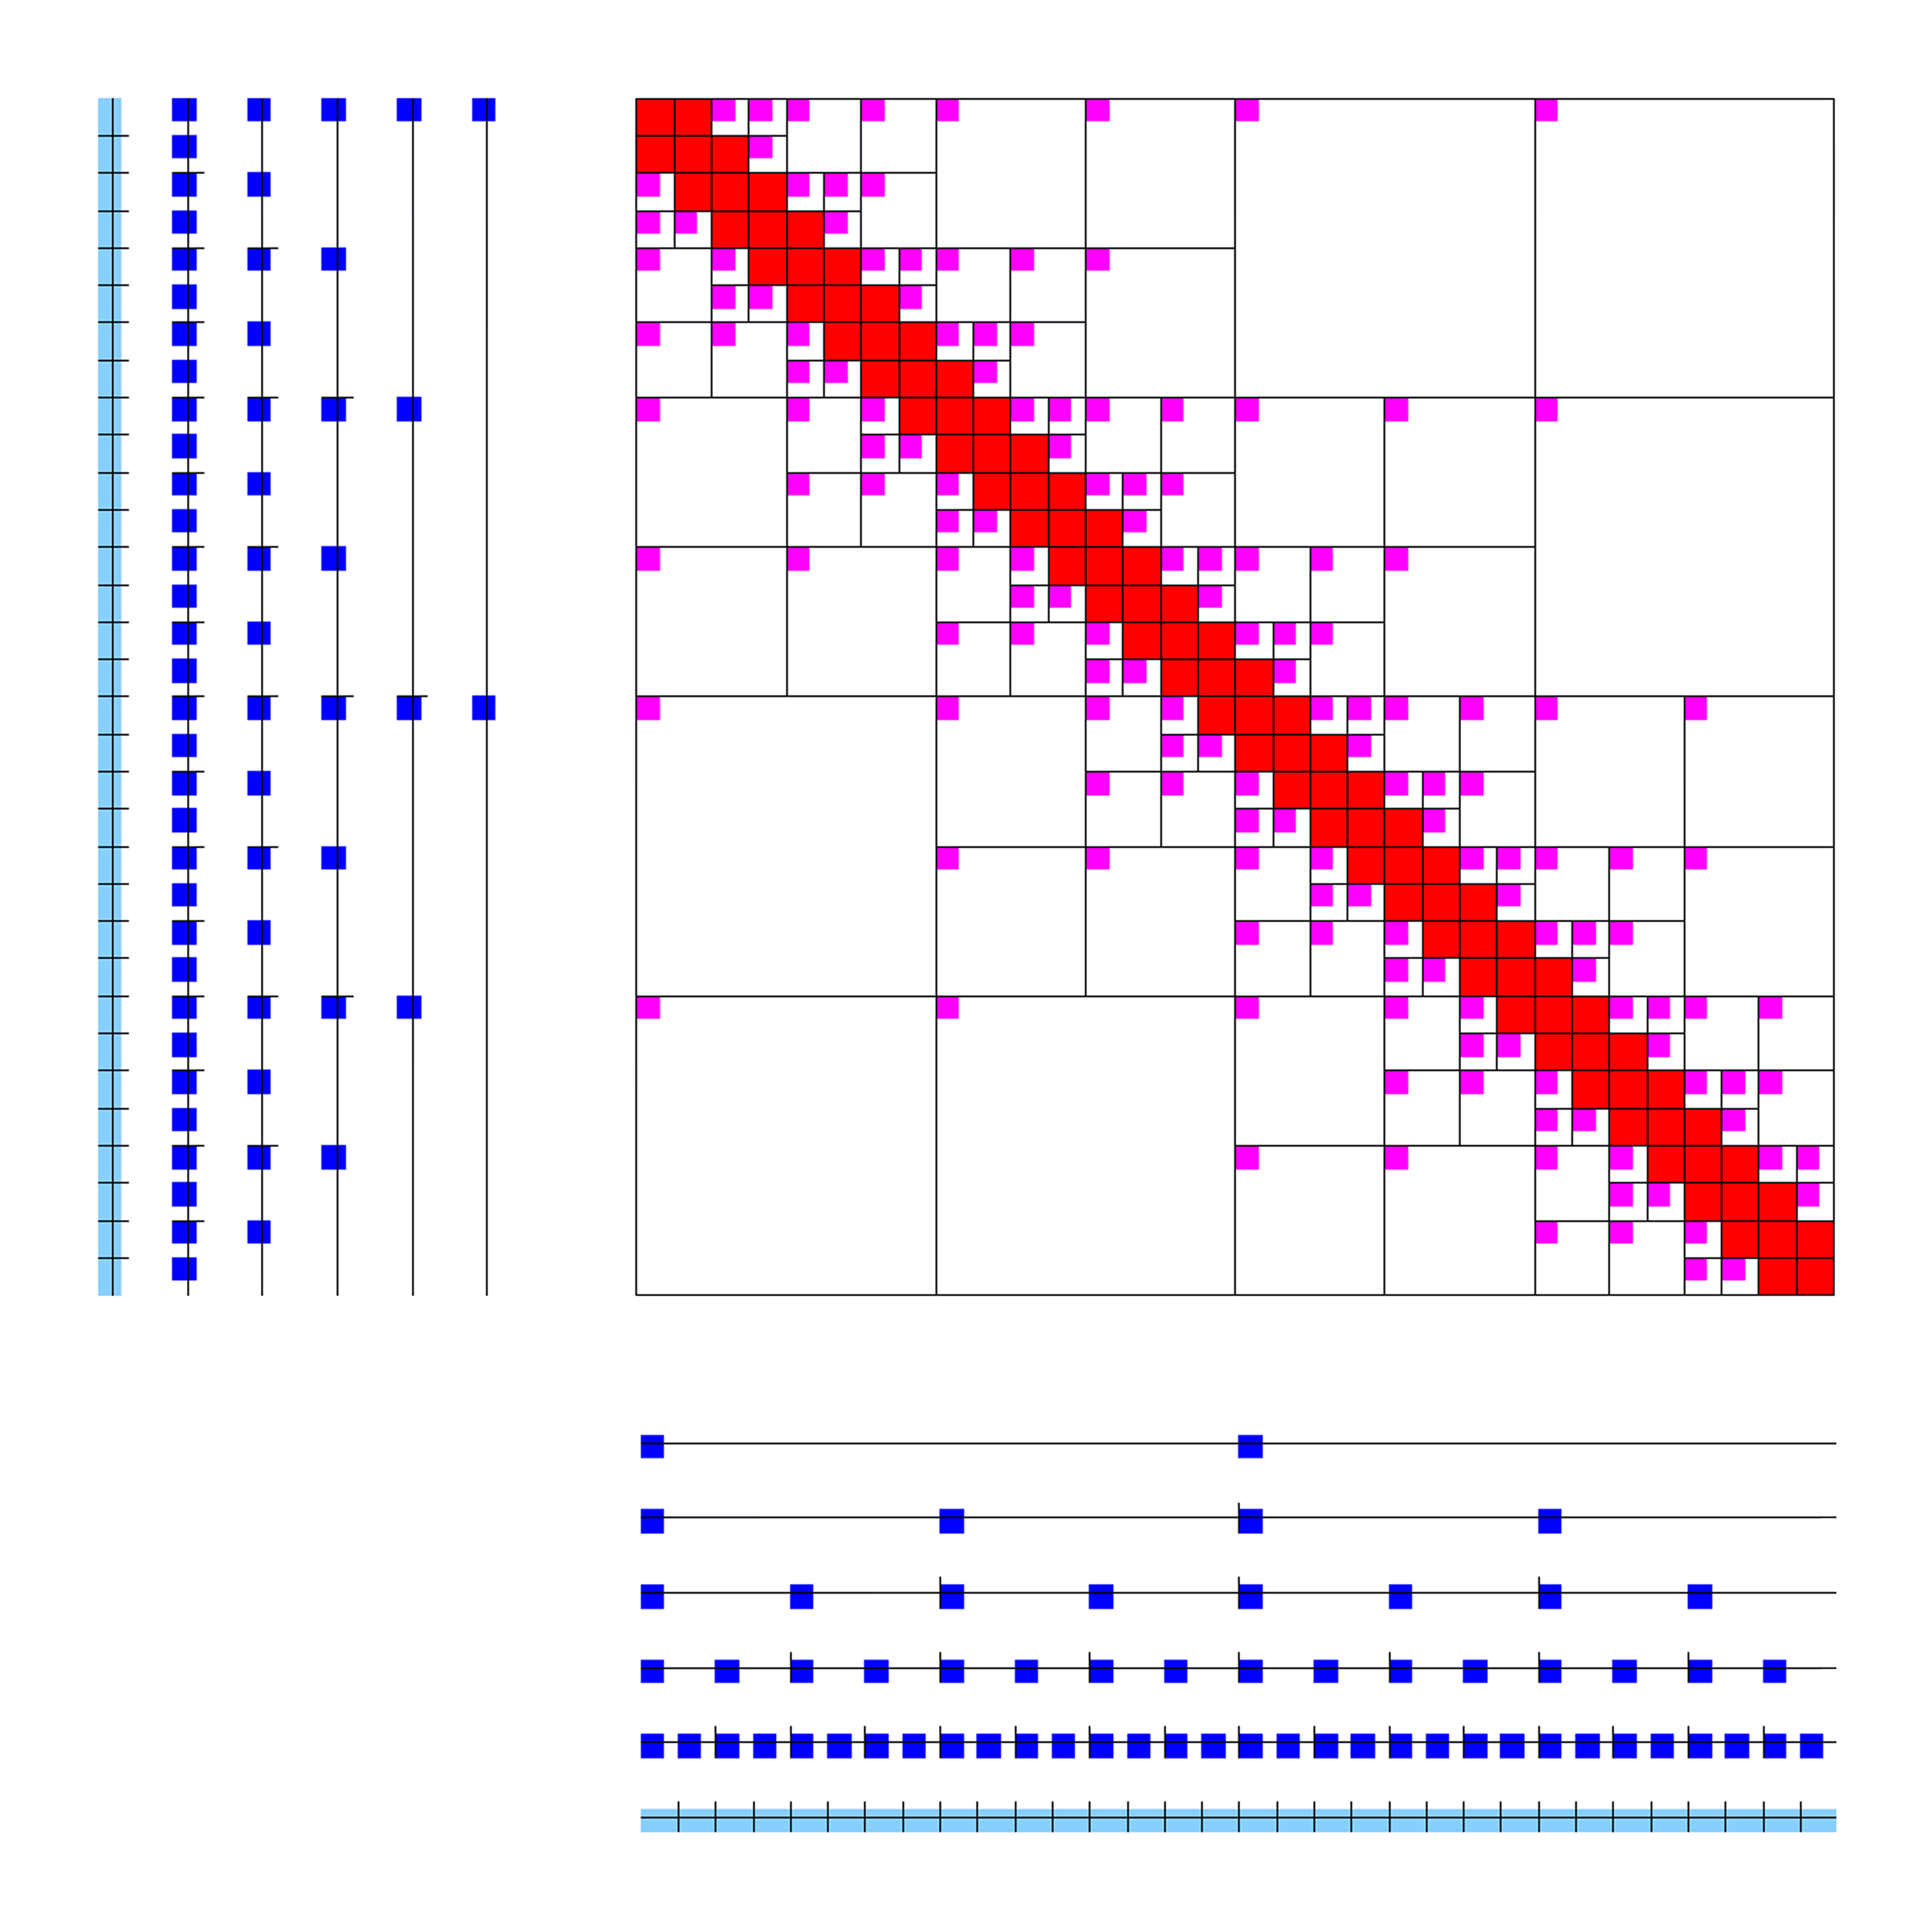
\includegraphics[width=0.7\textwidth]{img/h2-matrix.png}
      \caption{Darstellung einer $\mathcal{H}^2$-Matrix: In blau die geschachtelten Clusterbasen, in pink die Kopplungsmatrizen, in rot die verbleibenden Nahfeldmatrizen. (Quelle: \citet{h2slides})}
      \label{fig:h2}
    \end{figure}

    
      Die Überlegungen der letzten Abschnitte fließen nun in der Definition der \hquad zusammen.
      
      \begin{defn}
	(\hquad)\\
	Sei $T_{X \times Y}$ ein streng zulässiger Blockbaum, $k \in \N_0$ und seien $V$ und $W$ Clusterbasen des Ranges $k$ für die Clusterbäume $T_X$ und $T_Y$. Eine Matrix 
	$M \in \R^{X \times Y}$ heißt \textit{$\mathcal{H}^2$-Matrix} mit Zeilenbasis $V$ und Spaltenbasis $W$, falls für alle zulässigen Blattblöcke 
	$b = \tau \times \sigma \in \mathcal{L}^+\left(T_{X \times Y}\right)$ eine Matrix $S_b \in R^{k \times k}$ existiert, sodass
	\begin{equation*}
	  \left. M \right|_b = V_\tau S_b \trans{W_\sigma}
	\end{equation*}
	erfüllt ist. Die Familie $\left(S_b\right)_{b \in \mathcal{L}^+\left(T_{X \times Y}\right)}$ bezeichnen wir als Familie der \textit{Kopplungsmatrizen}.
      \end{defn}
      
      Für unzulässig Blattblöcke $b = \tau \times \sigma \in \mathcal{L}^-\left(T_{X \times Y}\right)$ verbleiben, wie auch bei den \hmat, die vollbesetzten Nahfeldmatrizen $N_b$.
      
      Mit geschachtelten Darstellungen 
      \[
      \left( 
	\left(V_\tau \right)_{\tau in \mathcal{L}\left(T_X\right)} , \left(E_\tau\right)_{\tau \in T_X \backslash \mathcal{L}\left(T_X\right)} \right) \text{ und }
	\left( \left(W_\sigma\right)_{\sigma in \mathcal{L}\left(T_Y\right)} , \left(F_\sigma\right)_{\sigma \in T_Y \backslash \mathcal{L}\left(T_Y\right)}
      \right) 
      \]
      der Clusterbasen $V$ und $W$ bezeichnen wir das Tupel
      \[
       \left(
	\left(S_b\right)_{b \in \mathcal{L}^+\left(T_{X \times Y}\right)} , \left(N_b\right)_{b \in \mathcal{L}^-\left(T_{X \times Y}\right)},
	\left(V_\tau\right)_{\tau in \mathcal{L}\left(T_X\right)} , \left(E_\tau\right)_{\tau \in T_X \backslash \mathcal{L}\left(T_X\right)},
	\left(W_\sigma\right)_{\sigma in \mathcal{L}\left(T_Y\right)} , \left(F_\sigma\right)_{\sigma \in T_Y \backslash \mathcal{L}\left(T_Y\right)}
       \right)
      \]
      als $\mathcal{H}^2$-Matrix-Darstellung der Matrix $M$.
      
      In \autoref{fig:h2} ist all dies zusammen dargestellt. Die Familien $\left(V_\tau\right)_{\tau in \mathcal{L}\left(T_X\right)}$ und $\left(W_\sigma\right)_{\sigma in \mathcal{L}\left(T_Y\right)}$
      links und unten sind hellblau gefärbt. Die Familien der Transfermatrizen $\left(E_\tau\right)_{\tau \in T_X \backslash \mathcal{L}\left(T_X\right)}$ und 
      $\left(F_\sigma\right)_{\sigma \in T_Y \backslash \mathcal{L}\left(T_Y\right)}$ sind in dunkelblau abgebildet. Die Kopplungsmatrizen $\left(S_b\right)_{b \in \mathcal{L}^+\left(T_{X \times Y}\right)}$
      sind in pink und die Nahfeldmatrizen $\left(N_b\right)_{b \in \mathcal{L}^-\left(T_{X \times Y}\right)}$ unverändert in rot dargestellt. Die Ersparnis an Speicherplatz gegenüber der vollbesetzten
      Matrix und selbst gegenüber der Darstellung als $\mathcal{H}$-Matrix ist augenscheinlich.

      Von \citet{datasparse} wird eine vollständige Charakterisierung der \hquad vorgenommen. Dadurch wird ein für uns entscheidender Unterschied zwischen \hmat und \hquad deutlich:
      Bei \hmat müssen die zu den zulässigen Blöcken $b =\tau \times \sigma \in \mathcal{L}^+\left(T_{X \times Y}\right)$ gehörige Matrizen $\left. M\right|_{\tau \times \sigma}$ niedrigen Rang besitzen.
      Bei \hquad hingegen müssen die deutlich größeren Matrizen $\left. M\right|_{\tau \times R_\tau}$ und $\left. M\right|_{C_\sigma \times \sigma}$ für alle Cluster $\tau \in T_X$ und $\sigma\in T_Y$
      niedrigen Rang besitzen. Dabei sind für alle $\tau \in T_X$ und $\sigma \in T_Y$ definiert:
      \[
	R_\tau := \bigcup_{r \in row*(\tau)} r , \ \ \ \ \ \ \ \ C_\sigma := \bigcup_{c \in col(\sigma)} c,
      \]
      \[
       row*(\tau) := \{ s \in T_Y \ | \ \exists \tilde \tau \in T_X \colon \ \tilde \tau \times s \in \mathcal{L}^+\left(T_{X \times Y}\right) \wedge \tau \in sons^*(\tilde \tau) \},
      \]
      \[
       \ col*(\sigma) := \{ t \in T_X \ | \ \exists \tilde \sigma \in T_Y \colon \ t \times \tilde \sigma \in \mathcal{L}^+\left(T_{X \times Y}\right) \wedge \sigma \in sons^*(\tilde \sigma) \}.
      \]
      Dieser Unterschied ist in \autoref{fig:hh2diff} bildlich dargestellt:
      
      \begin{figure}[b]
	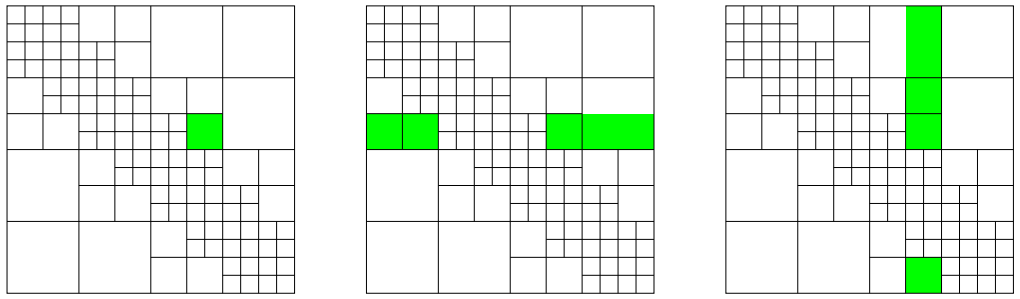
\includegraphics[width=\textwidth]{img/H_H2_diff.png}
	\caption{Vergleich zwischen $\mathcal{H}$- und $\mathcal{H}^2$-Matrix: Bei ersterer müssen nur einzelne Teilmatrizen niedrigen Rang besitzen, bei letzterer ganze Zeilen- und Spaltenblöcke.
	(Quelle: \citet{nichtlokop})}
	\label{fig:hh2diff}
      \end{figure}


      Mit den \hquad haben wir also eine sehr effiziente Teilmenge der hierarchischen Matrizen gefunden, die sich noch kompakter speichern lassen und mit denen Berechnungen noch effizienter 
      durchgeführt werden können.